\chapter{Testing and Results}
In order to test the system a series of tests were conducted to test each system individually before the overall system was tested. The individual systems tested are the GPS and compass, the PWM output, throttle, and the individual thrusters. Finally the full system was tested on the Stellenbosch canoe dam. 
\section{GPS and Compass}
The GPS and compass were tested on land. A baseline was established using a tracking application on a cellphone. The GPS and compass together with the cellphone were placed in a bag and a route was walked. The tracking data from both sources can then be downloaded and formatted as a Keyhole Markup Language (.kml) file and displayed on a map or plotted as has been done in figure \ref{fig:4:GPSMap}.\par
\begin{figure}
	\begin{center}
		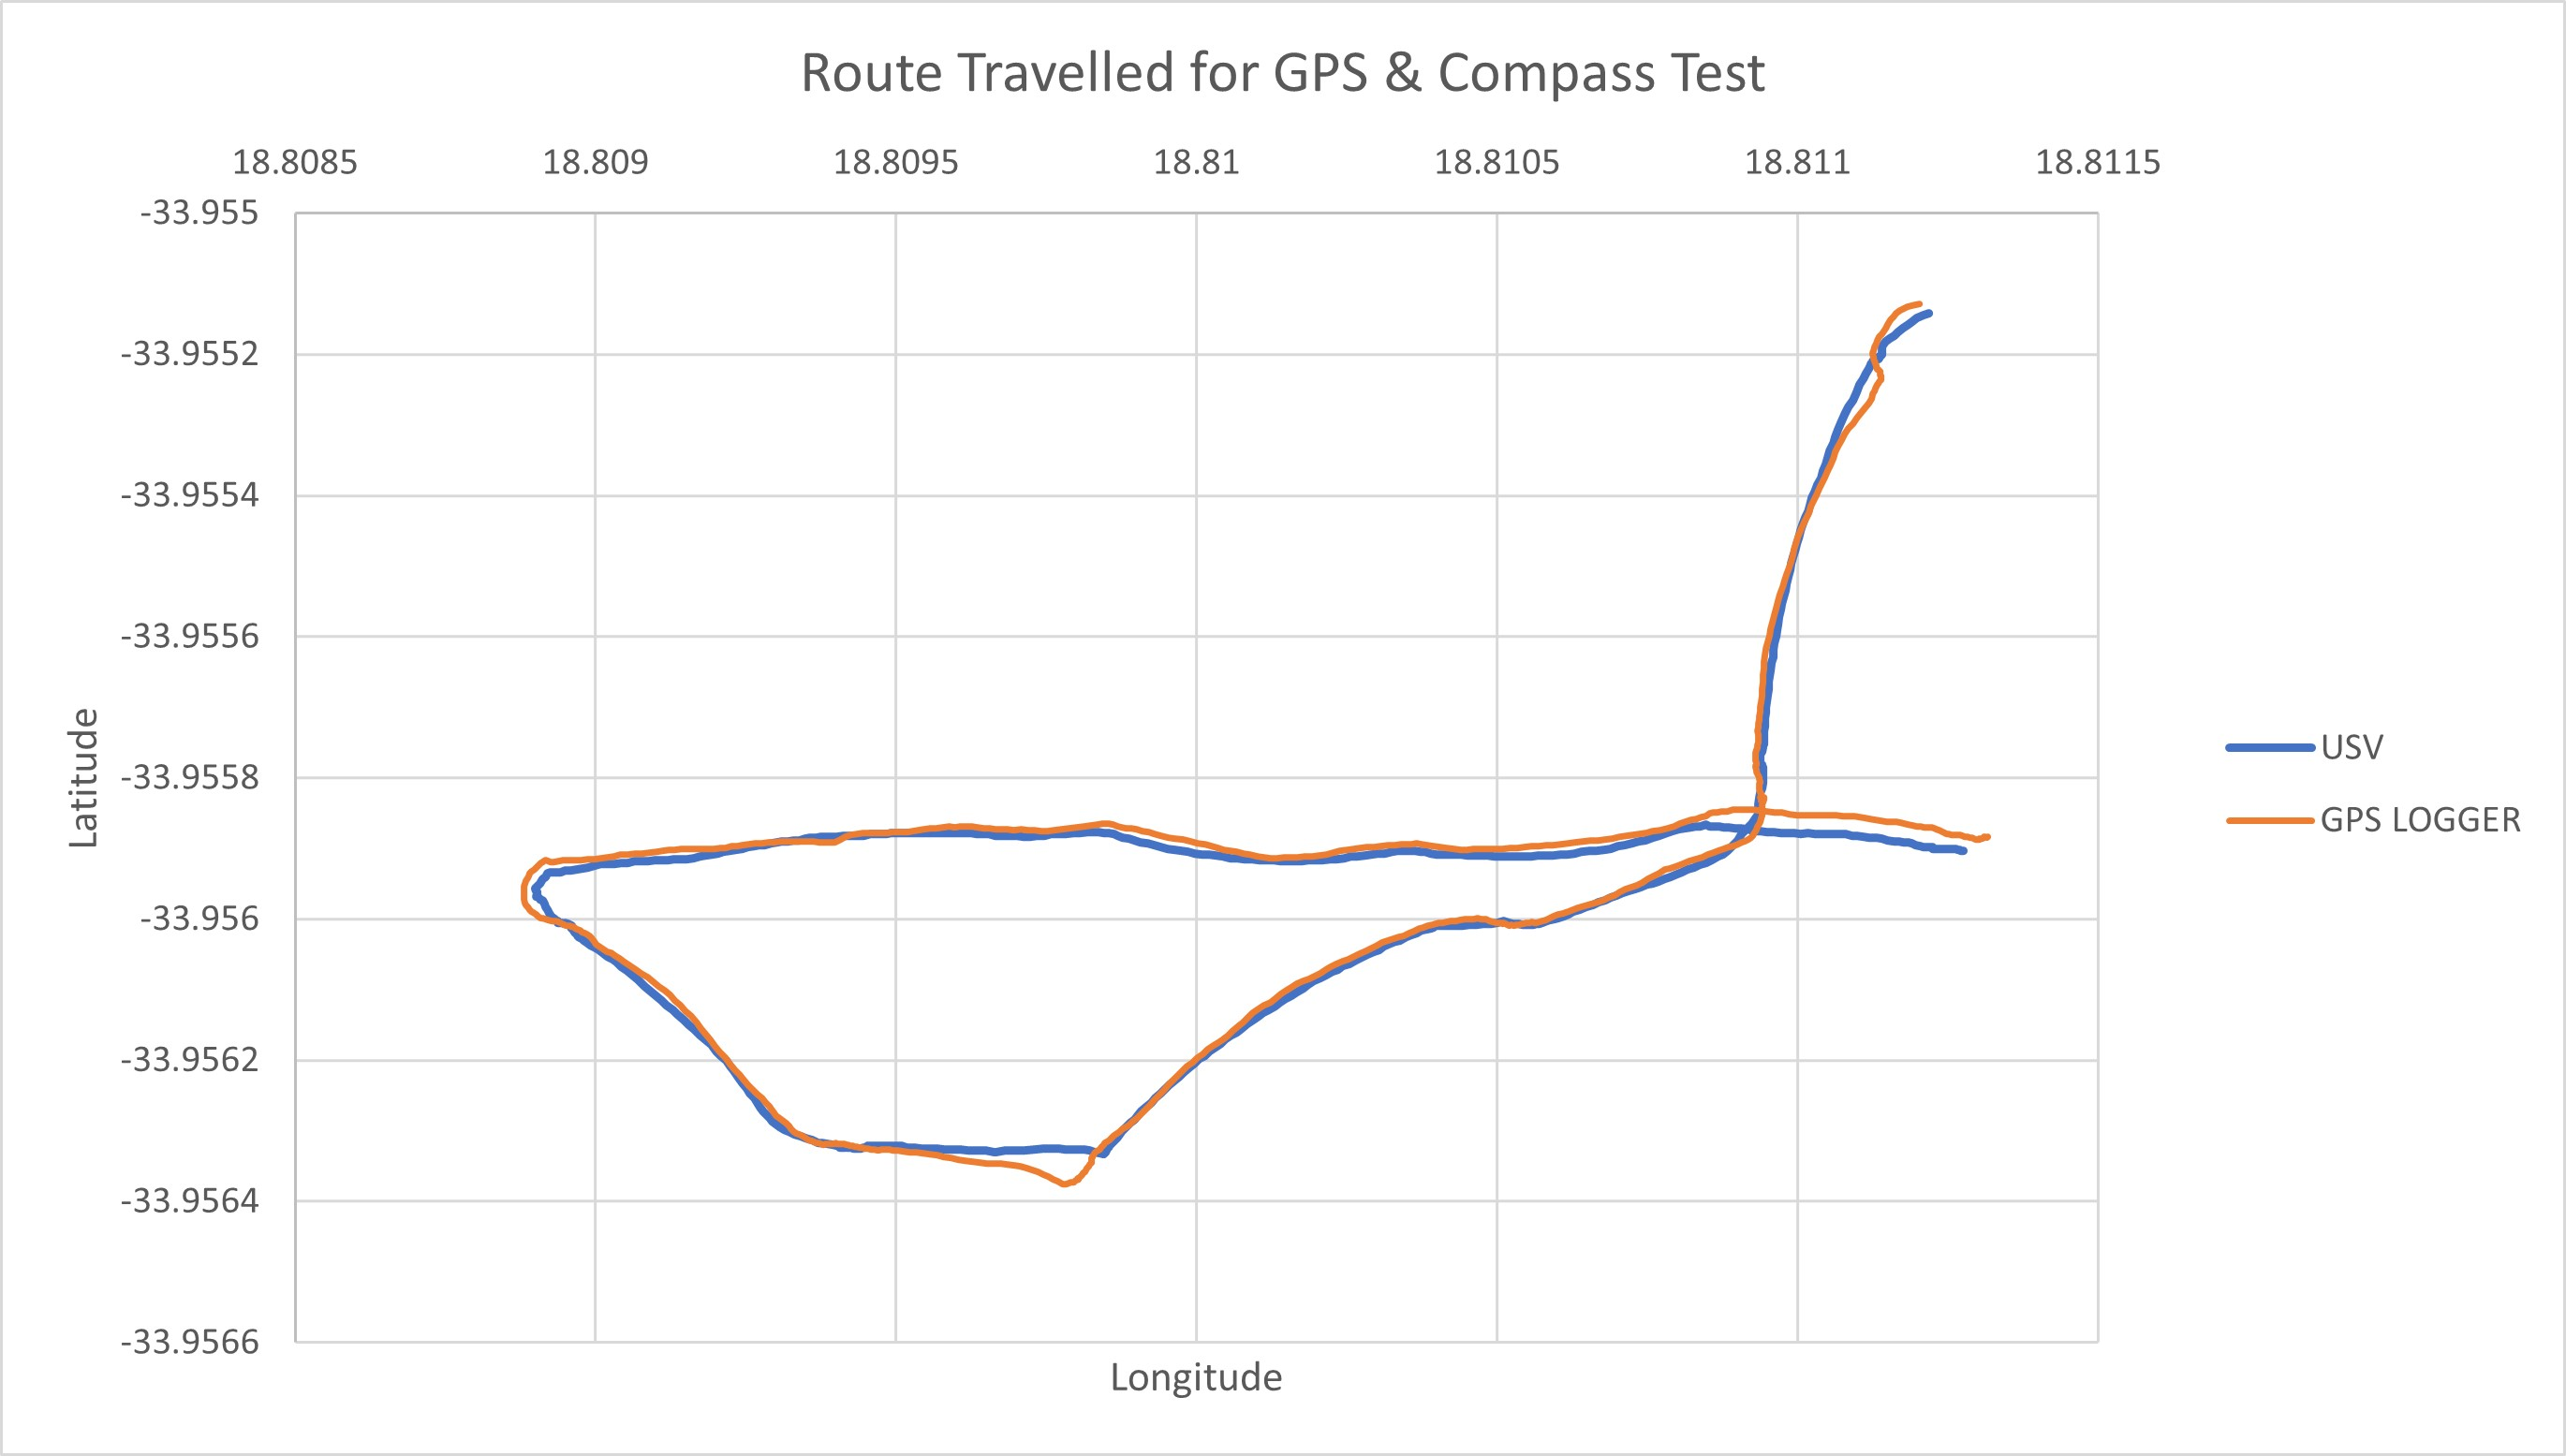
\includegraphics[width=0.8\linewidth]{figures/graphGPSMap.jpg}
		\caption{The path used to compare the system GPS and the baseline GPS logger.}
		\label{fig:4:GPSMap}
	\end{center}
\end{figure}
In order to have a bearing to compare the compass reading with, the last two GPS points were used to calculate the bearin on which the vessel is pointing. Figure \ref{fig:4:bearingTest} shows the calculated bearing and the GPS bearing plotted together.\par
\begin{figure}
	\begin{center}
		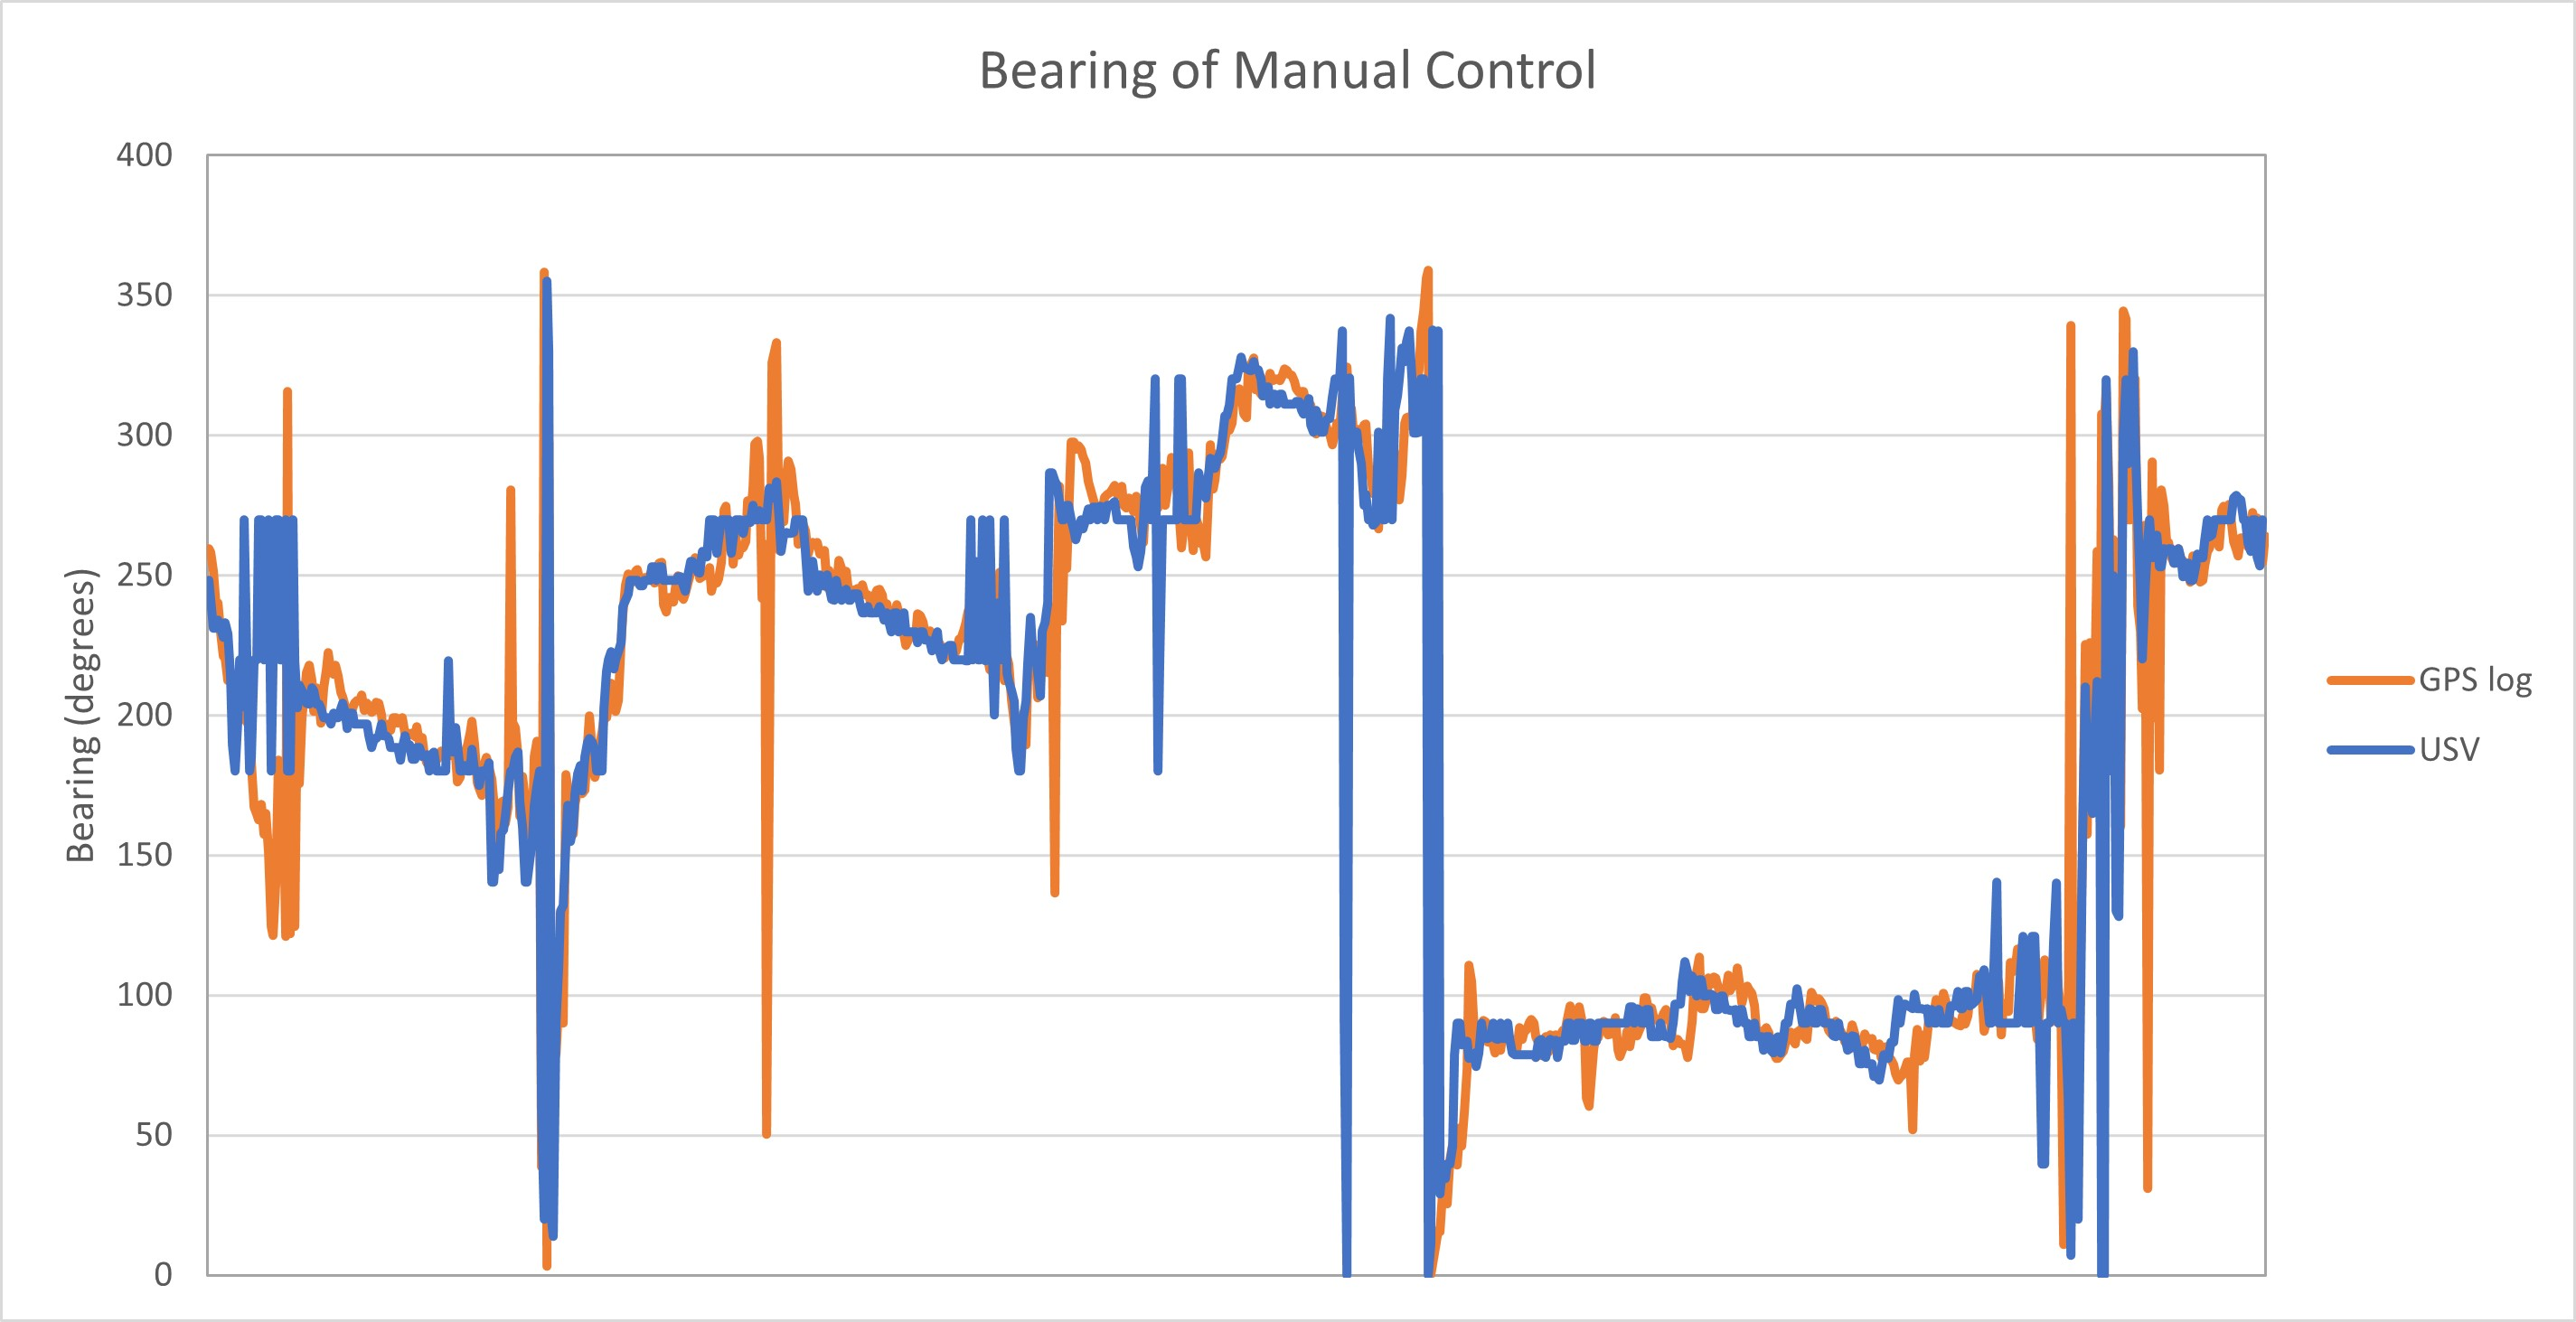
\includegraphics[width=0.8\linewidth]{figures/graphBearingManual.jpg}
		\caption{The calculated bearing and compass bearing overlay.}
		\label{fig:4:bearingTest}
	\end{center}
\end{figure}
As can be seen in figure \ref{fig:4:GPSMap}, the two sets of GPS data match each other very closely with only a few areas where the systems GPS moves away from the baseline GPS points. In order to quantify the accuracy of the GPS, the distance between the coinciding points of the baseline GPS and the system GPS was calculated and plotted on box and whisker chart of figure \ref{fig:4:GpsBxWh}. As you can see the GPS is accurate to within \SI{5}{\meter} with only a few outliers, making up less than \SI{4}{\percent} of the data, falling slightly outside the \SI{5}{\meter} mark.\par
Similarly it can be seen on figure \ref{fig:4:bearingTest} that the systems compass bearing is closely following the calculated baseline bearing. Figure \ref{fig:4:bearingBxWh} shows a box and whisker plot of the error between the two bearings, with most of the data falling within a \SI{20}{\degree} range. There are more outliers than in the GPS test, however this is due to calculated bearing having several spikes. These spikes occur when the because the bearing is being calculated between GPS points that are often within 1m of each other and some accuracy can be lost. The noticeable spike of the system compass in figure \ref{fig:4:bearingTest} is not an error but caused by the bearing going around passed \SI{360}{\degree} to \SI{0}{\degree}.
 \begin{figure}[!hb]
 	\begin{center}
 		\begin{subfigure}{0.45\linewidth}
 			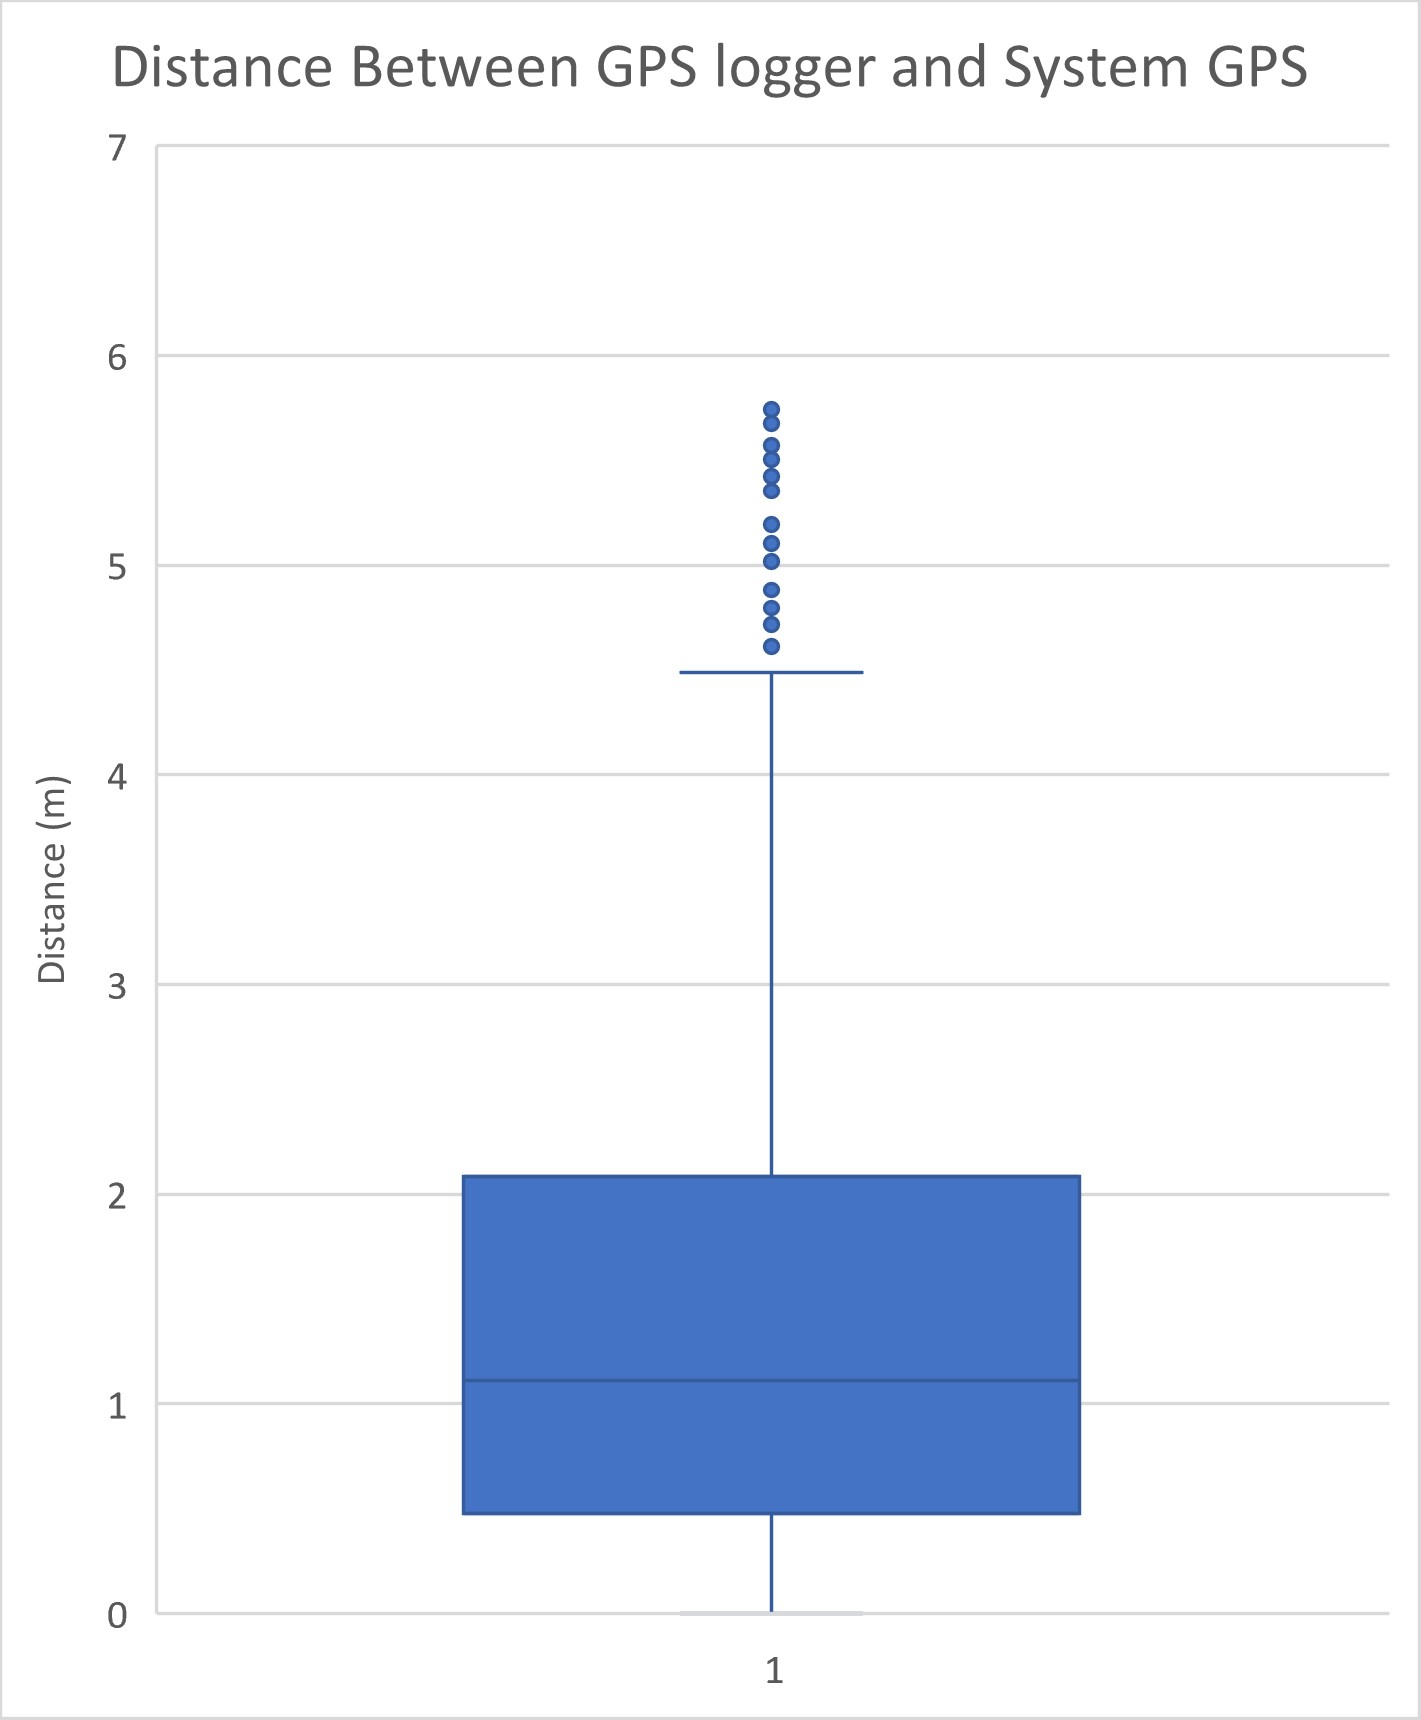
\includegraphics[width = \linewidth]{figures/distBxWh.jpg}
 			\caption{Distance.}
 			\label{fig:4:GpsBxWh}	
 		\end{subfigure}
 		\begin{subfigure}{0.475\linewidth}
 			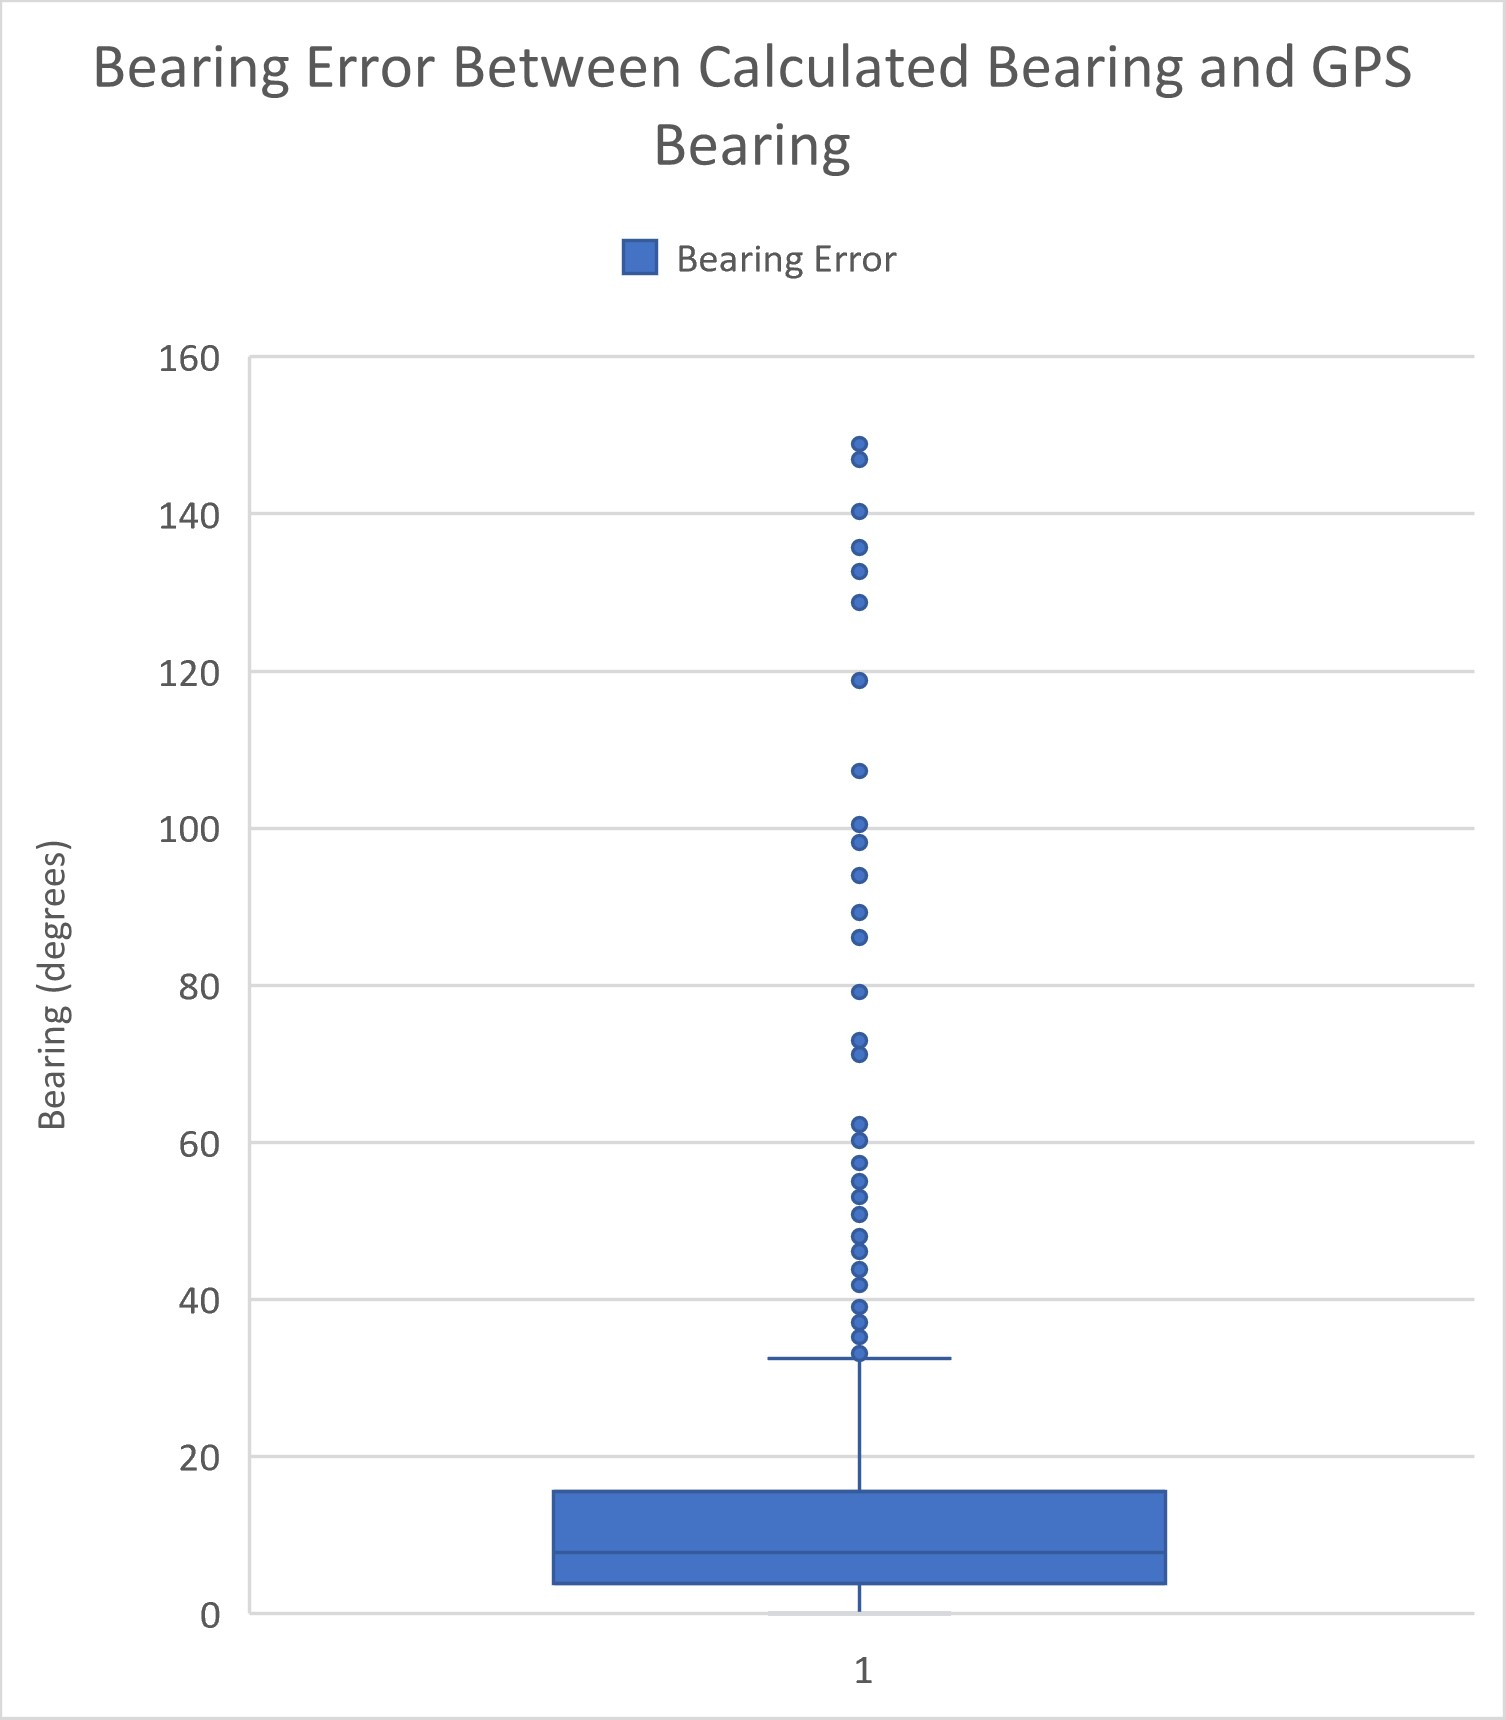
\includegraphics[width = \linewidth]{figures/bearingBxWh.jpg}
 			\caption{Bearing}
 			\label{fig:4:bearingBxWh}	
 		\end{subfigure}
 	\caption{Box and Whisker Graphs Of Distance and Bearing Between the System and the Baseline.}
 	\end{center}
 \end{figure} 
\section{PWM Output}
In order to adjust the speed of the thrusters, the PWM output must vary based on the throttle input. The PWM signal can easily be measured using an oscilloscope, therefore the system was set-up as shown in figure \ref{fig:4:PWMTest}. The throttle was connected to microcontrollers analogue inputs as it would be for the full system. The PWM outputs where then attached to the oscilloscope probes and the Arduino native programming port was used to power the system from a laptop. Each PWM signal was first tested individually before finally, both signals were tested simultaneously, each one on its own channel. \par
\begin{figure}
	\begin{center}
		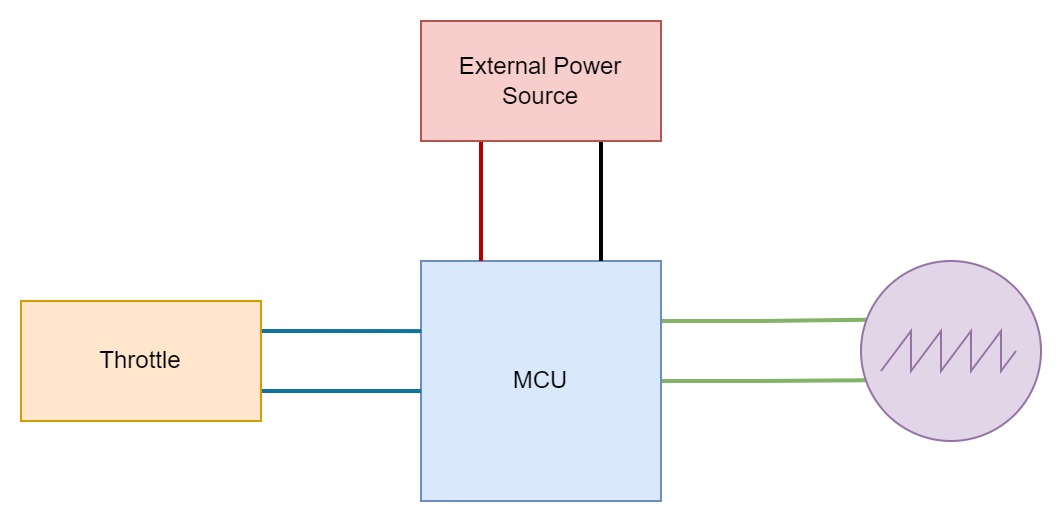
\includegraphics[width=0.6\linewidth]{figures/PWMtest.jpg}
		\caption{Wiring diagram for the PWM oscilloscope test.}
		\label{fig:4:PWMTest}
	\end{center}
\end{figure}
As the throttle is adjusted the PWM signal should vary. There are three distinct positions, full forward, neutral and full reverse. that can be noted in table \ref{tab:3:PWM}. Theses three positions were tested to ensure that the range of the throttle was correctly calibrated. Finally the PWM signal was observed while slowly adjusting the throttle to ensure that the PWM signal varied linearly and in with a timely response. The results of the oscilloscope test are shown in figure \ref{fig:4:OscTest}. \par
It can be seen that the PWM responded well to the throttle inputs and met all three of the notable positions perfectly. Figure \ref{fig:4:OscTest:both} also shows that the two PWM outputs can have independent values to control each thruster as required. It should be noted that the images in figure \ref{fig:4:OscTest} all show a amplitude of \SI{3.3}{\volt} as the output was measured directly off of the Arduino microcontroller and before the signal was amplified using the logic level converter. It was confirmed that the converter accurately amplified the signal while maintaining the frequency and duty cycle of the signal.
\begin{figure}
	\begin{center}
		\begin{subfigure}{0.47\linewidth}
			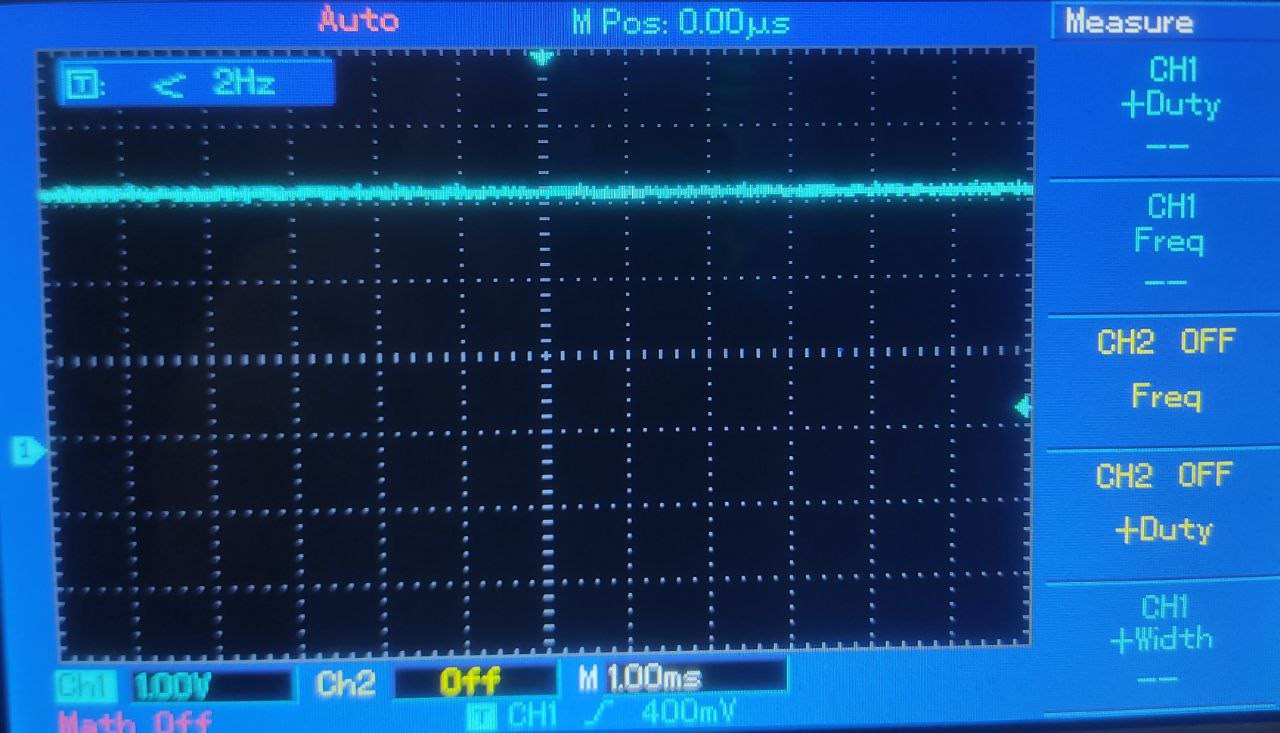
\includegraphics[width = \linewidth]{figures/PWMfoward.jpg}
			\caption{Full Forward}
			\label{fig:4:OscTest:forward}	
		\end{subfigure}
		\begin{subfigure}{0.47\linewidth}
			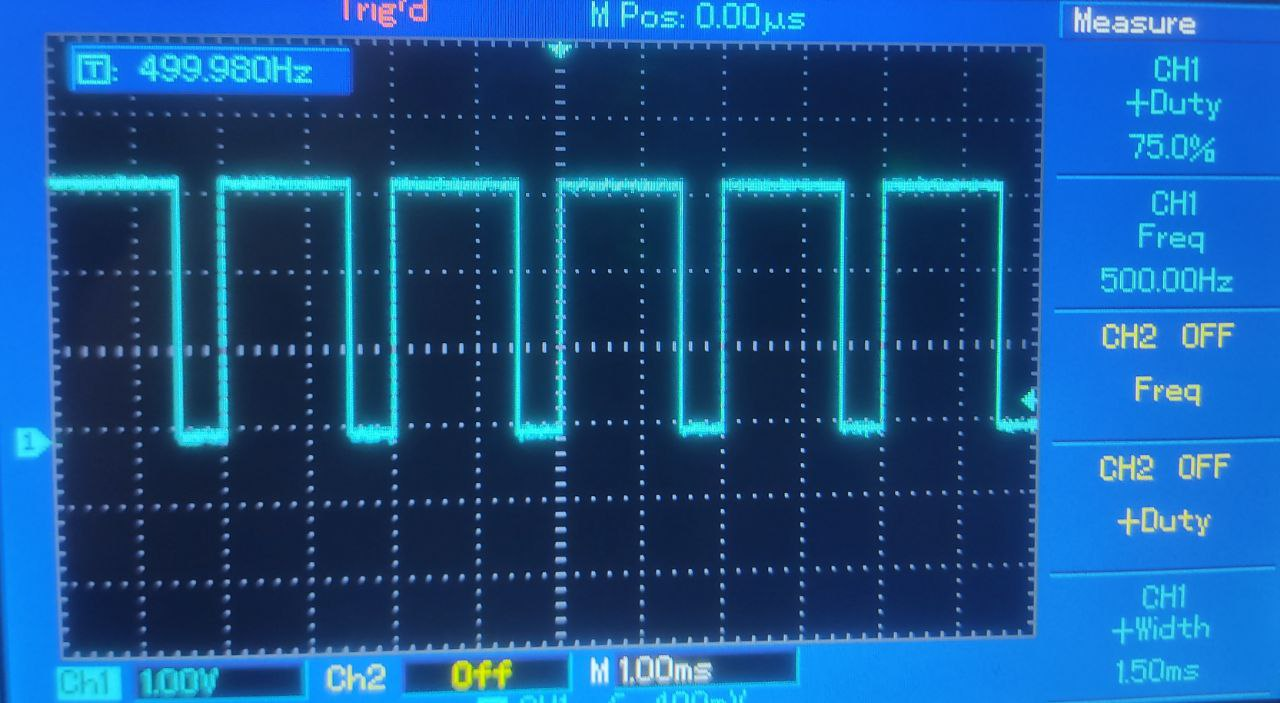
\includegraphics[width = \linewidth]{figures/PWMneutral.jpg}
			\caption{Neutral}
			\label{fig:4:OscTest:neutral}	
		\end{subfigure}
		\begin{subfigure}{0.47\linewidth}
			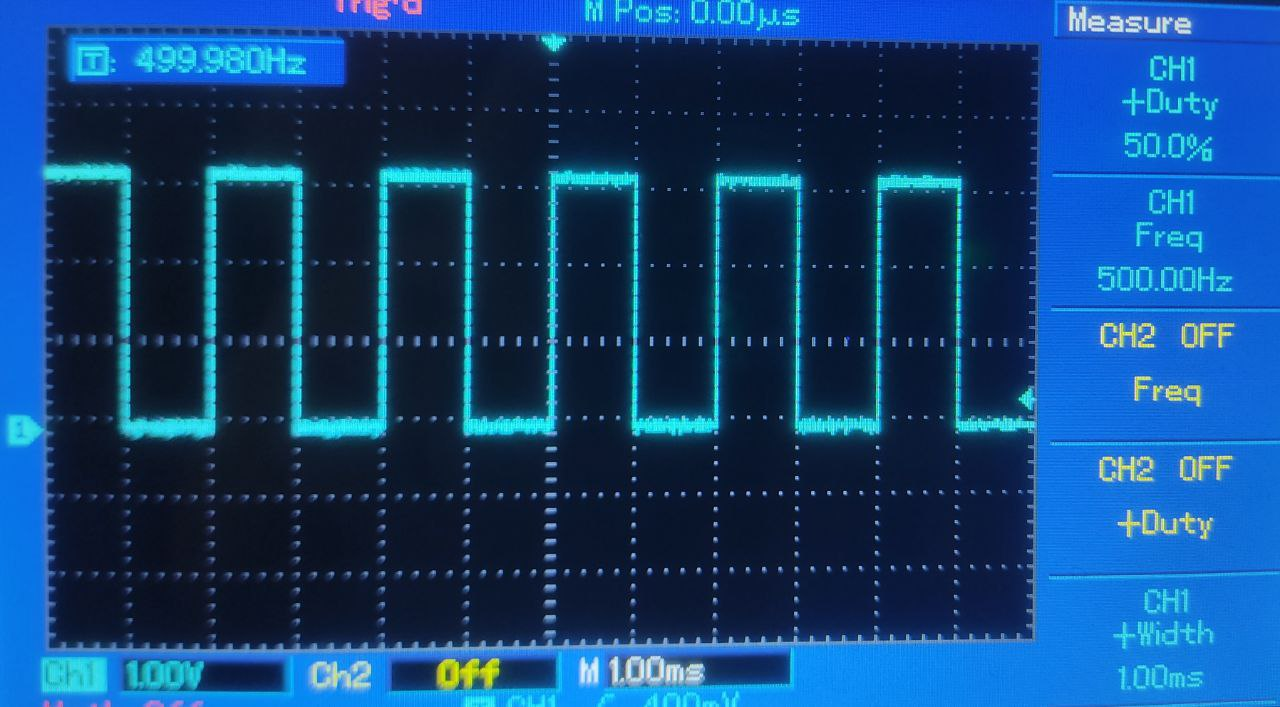
\includegraphics[width = \linewidth]{figures/PWMreverse.jpg}
			\caption{Full Reverse}
			\label{fig:4:OscTest:reverse}	
		\end{subfigure}
		\begin{subfigure}{0.47\linewidth}
			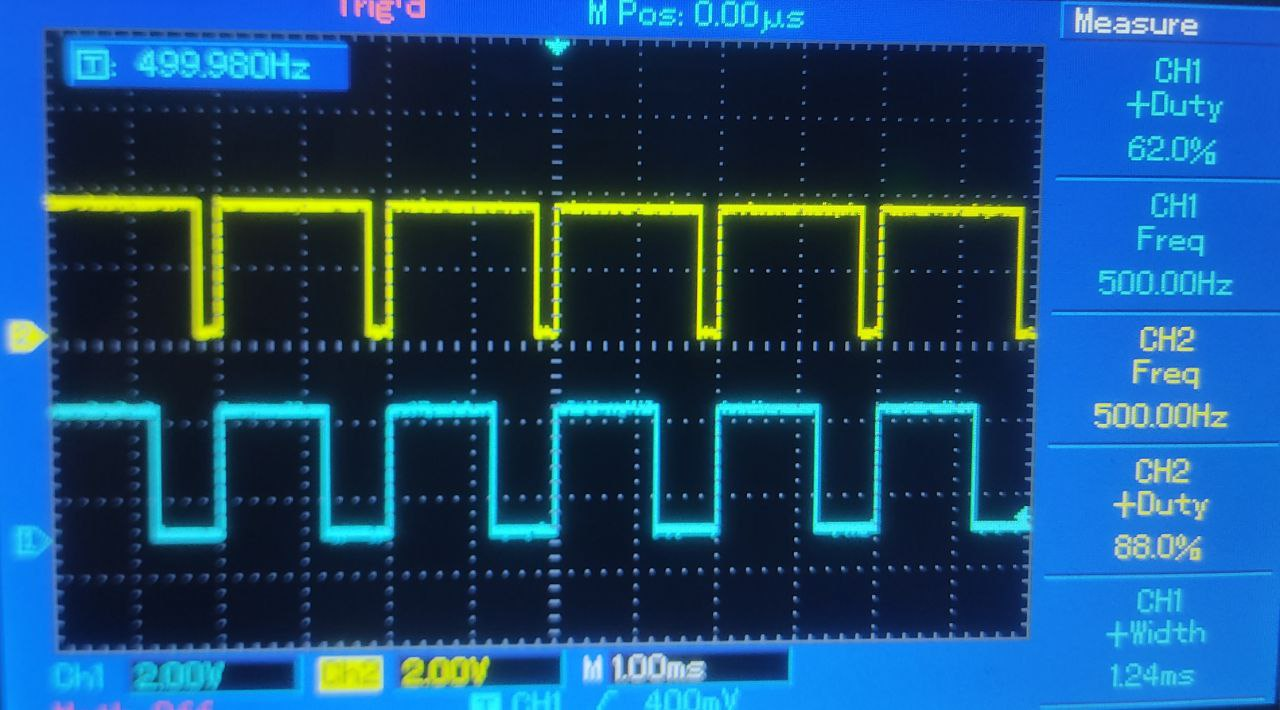
\includegraphics[width = \linewidth]{figures/PWMboth.jpg}
			\caption{Both Outputs}
			\label{fig:4:OscTest:both}	
		\end{subfigure}
		\caption{Results of the PWM output displayed on an oscilloscope.}
		\label{fig:4:OscTest}
	\end{center}
\end{figure} 
\section{Throttle}
\begin{figure}
	\begin{center}
		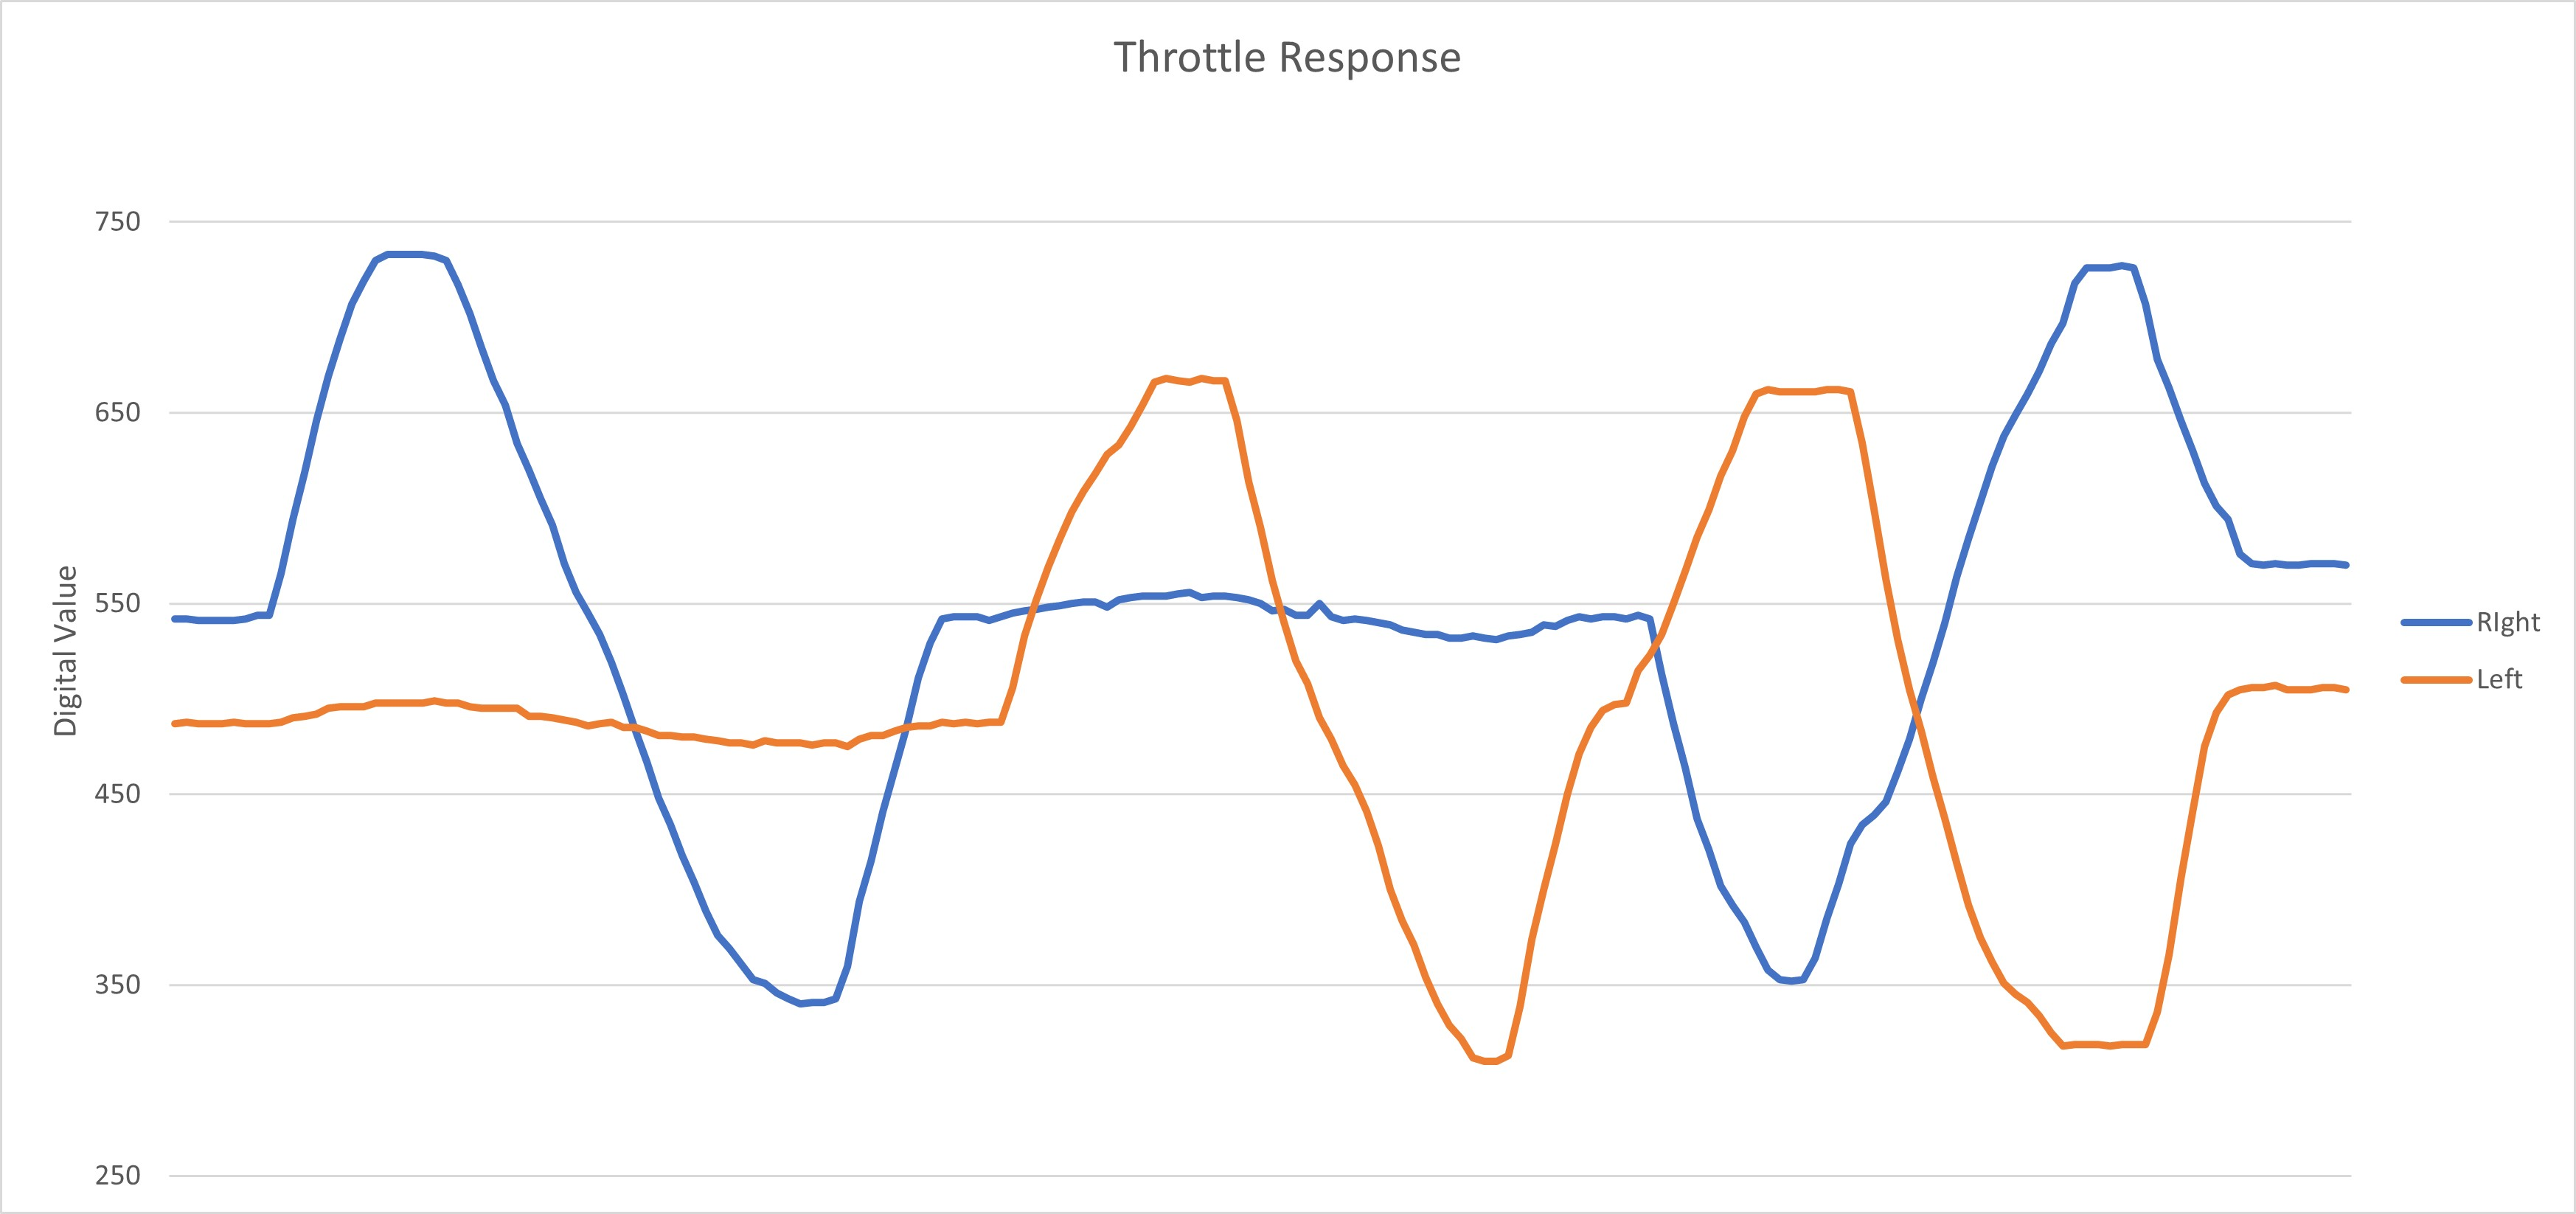
\includegraphics[width = 0.8\linewidth]{figures/graphThrottle.jpg}
		\caption{The digital response of the throttle.}
		\label{fig:4:Throttleresponse}
	\end{center}
\end{figure}
In order to test the response of the throttle and to show that the linear potentiometers have good accuracy the graph in \ref{fig:4:Throttleresponse} was plotted. It can clearly be seen that the potentiometers are meeting the upper and lower thresholds listed in \ref{tab:3:POT} and can move independently of each other without interference. Figure \ref{fig:4:Throttleresponse} also shows that in the neutral position there is some variation caused by user input when moving the other throttle. As one pushes on the one throttle one, will slightly pull on the other without realizing. Furthermore, even if it looks like the throttle is back in the neutral position, even a small amount off from the original position results in a different value. This is why the neutral buffer in \ref{tab:3:POT} was applied and it can be seen that buffer covers the slight variations. 
\begin{figure}
	\begin{center}
		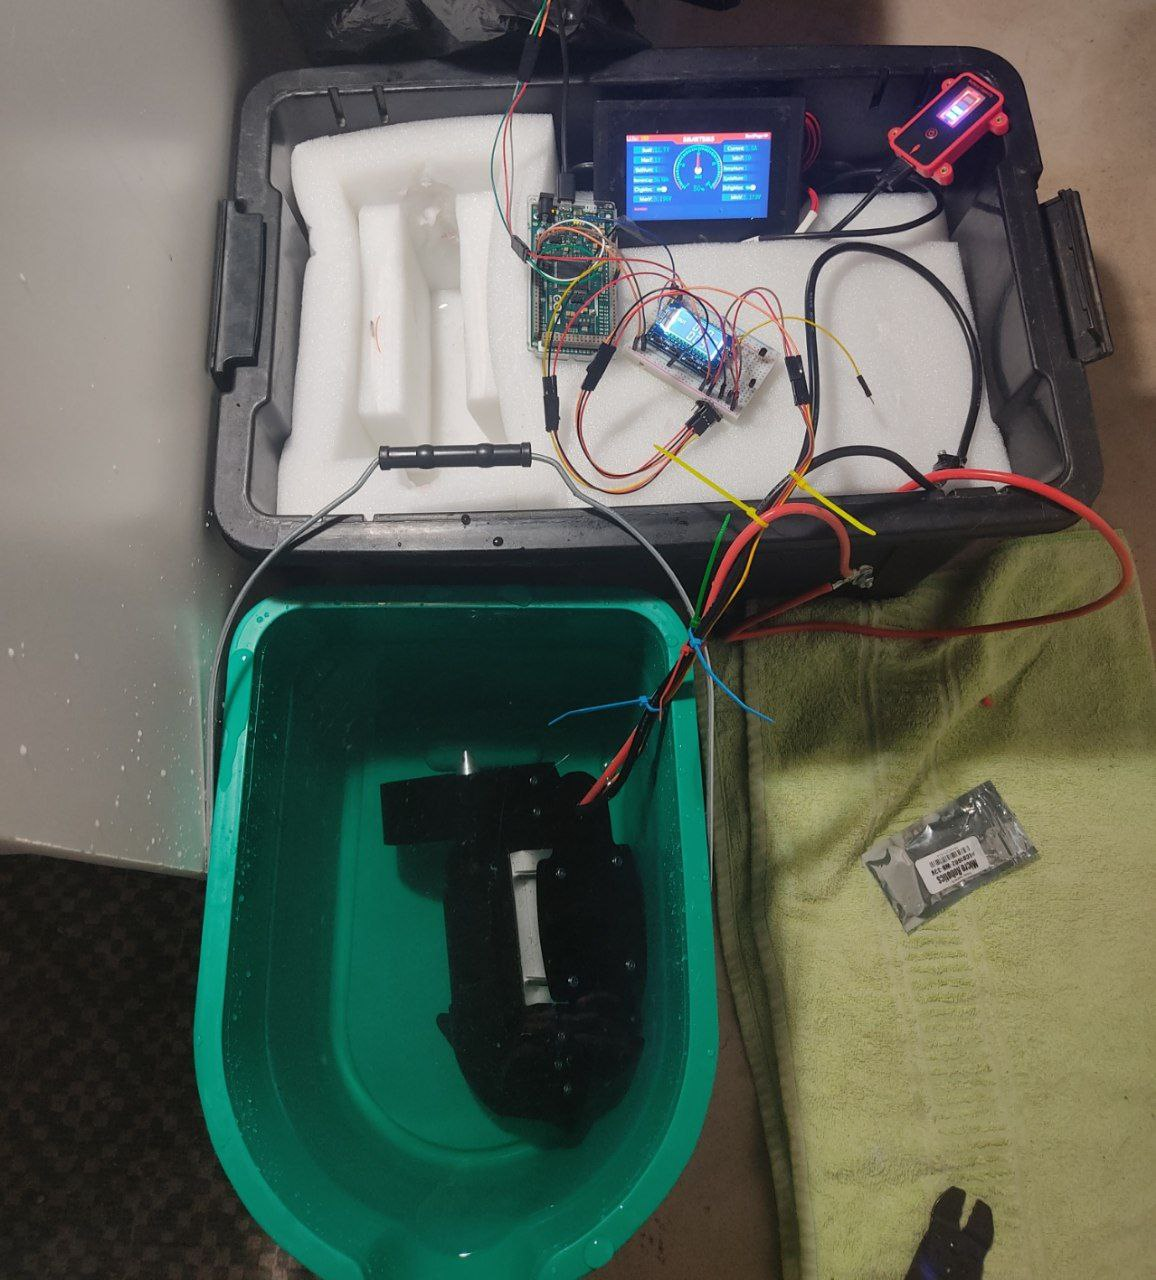
\includegraphics[width = 0.45\linewidth]{figures/thrusterBucket.jpg}
		\caption{The thruster in a bucket of water to test it without 'dry running'.}
		\label{fig:4:ThrusterTest}
	\end{center}
\end{figure}
\section{Thrusters}
The thrusters are designed to be operated in water as the water flow across the ESC is designed to dissipate the heat generated and prevent the ESC from overheating. Furthermore, the thruster is designed to push water and not air which have very different densities, so for these reasons the thrusters should not be 'dry run', and should only be operated while submerged. Figure \ref{fig:4:ThrusterTest} shows how, during the design and testing of the thrusters, a temporary water source was provide with a large bucket wherein the thrusters could be submerged to ensure that the thruster is responding to the PWM signal and giving the desired results.

\section{USV}
The final testing was conducted on the entire system as a whole by launching the vessel and operating it as a complete system. This section will first detail the procedure for setting up the system for a test followed by the details of how each test was carried out. Finally, the results of the full system tests will be discussed. 
\subsection{Set-up Procedure} 
The full system tests were carried out on the Stellenbosch canoe dam as it is a large enough body of water to sufficiently test the vessel and it is just outside of Stellenbosch so it is easily accessible. The system is transported completely disassembled so as to avoid any possible damages that could occur during transport. Therefore, before testing the vessel as well as the rest of the components must be set-up and checked before the vessel can be launched and the test can begin. Firstly the vessel and all safety equipment must be checked and prepared by following the checklist in table \ref{tab:4:boatCheck}. Once the vessel has be prepared the system can be assembled by following the checklist in table \ref{tab:4:equipCheck}. Once both of these checklists have been followed a final cursory sweep should be conducted to ensure that nothing has been missed and the vessel can be launched. Once the vessel is off of the trailer and in the water, the thrusters can be dropped down into their operational position. This will conclude the set-up of the vessel and the test can begin. 
\begin{table}
	\begin{center}
		
		\caption{Procedure to set-up the vessel and safety equipment}
		\label{tab:4:boatCheck}
		\begin{tabular}{|l|l|}
			\hline
			To Check: & Checked \\
			\hline
			All bungs are in place and secured. &\\
			\hline
			All tie downs are removed and stowed. &\\
			\hline
			The personal floatation device is aboard. &\\
			\hline
			The electrical fire extinguisher is aboard. &\\
			\hline
			There is no physical damage to the vessel that could cause leaks.&\\
			\hline
		\end{tabular}
	\end{center}
\end{table}
 \begin{table}
 	\begin{center}
 		\caption{Procedure to set-up the equipment and control system}
 		\label{tab:4:equipCheck}
 		\begin{tabular}{|p{0.65\linewidth}|l|}
			\hline
 			To Check: & Checked \\
 			\hline
 			Mount the throttle plate and secure the attaching bolts.&\\
 			\hline
 			Mount the control system under the throttle plate and secure the GPS and Compass onto the nose.&\\
 			\hline
 			Ensure that the thrusters are in the upright position and mount them onto the transom.&\\
 			\hline
 			Place the batteries at the back of the vessel, just in front of the transom.&\\
 			\hline
 			Ensure that the cut-off switch is in the off position and connect the thrusters to the batteries.&\\
 			\hline
 			Connect the control system to the thrusters. &\\
 			\hline
 			Check all connections to see that they are secure and that there are no open wires. &\\
 			\hline
 			Close the battery box and secure the battery box. &\\
 			\hline
 			Turn on the cut-off switch to power the system and check that the control system powers on. The thrusters should beep twice signifying that they are connected and receiving a signal.&\\
 			\hline
 			Wait until the GPS indicator light is on, signifying that the GPS has an valid GPS fix. &\\
 			\hline
 		\end{tabular}
 	\end{center}
 \end{table}
\subsection{Testing}
The testing occurred in two phases, the manual test and the autonomous test. The manual test was carried out by using the throttle to manually control the vessel and ensure that the thrusters are responding correctly and that the system is fully operational. The GPS points that the boat would navigate to under autonomous control were chosen while doing the manual test to ensure that the vessel would not navigate into any of the obstacles on the dam such as buoys and pumps.\par
Finally, for the autonomous test, the vessel was driven back to the starting position and the system was reset and autonomous navigation was selected. The vessel was still manned so that manual control could be taken at any point if it looked as though the vessel would collide with any obstacles. Once the vessel had navigated to its final point, manual control was selected to return the vessel to shore. 
\begin{figure}[!hb]
	\begin{center}
		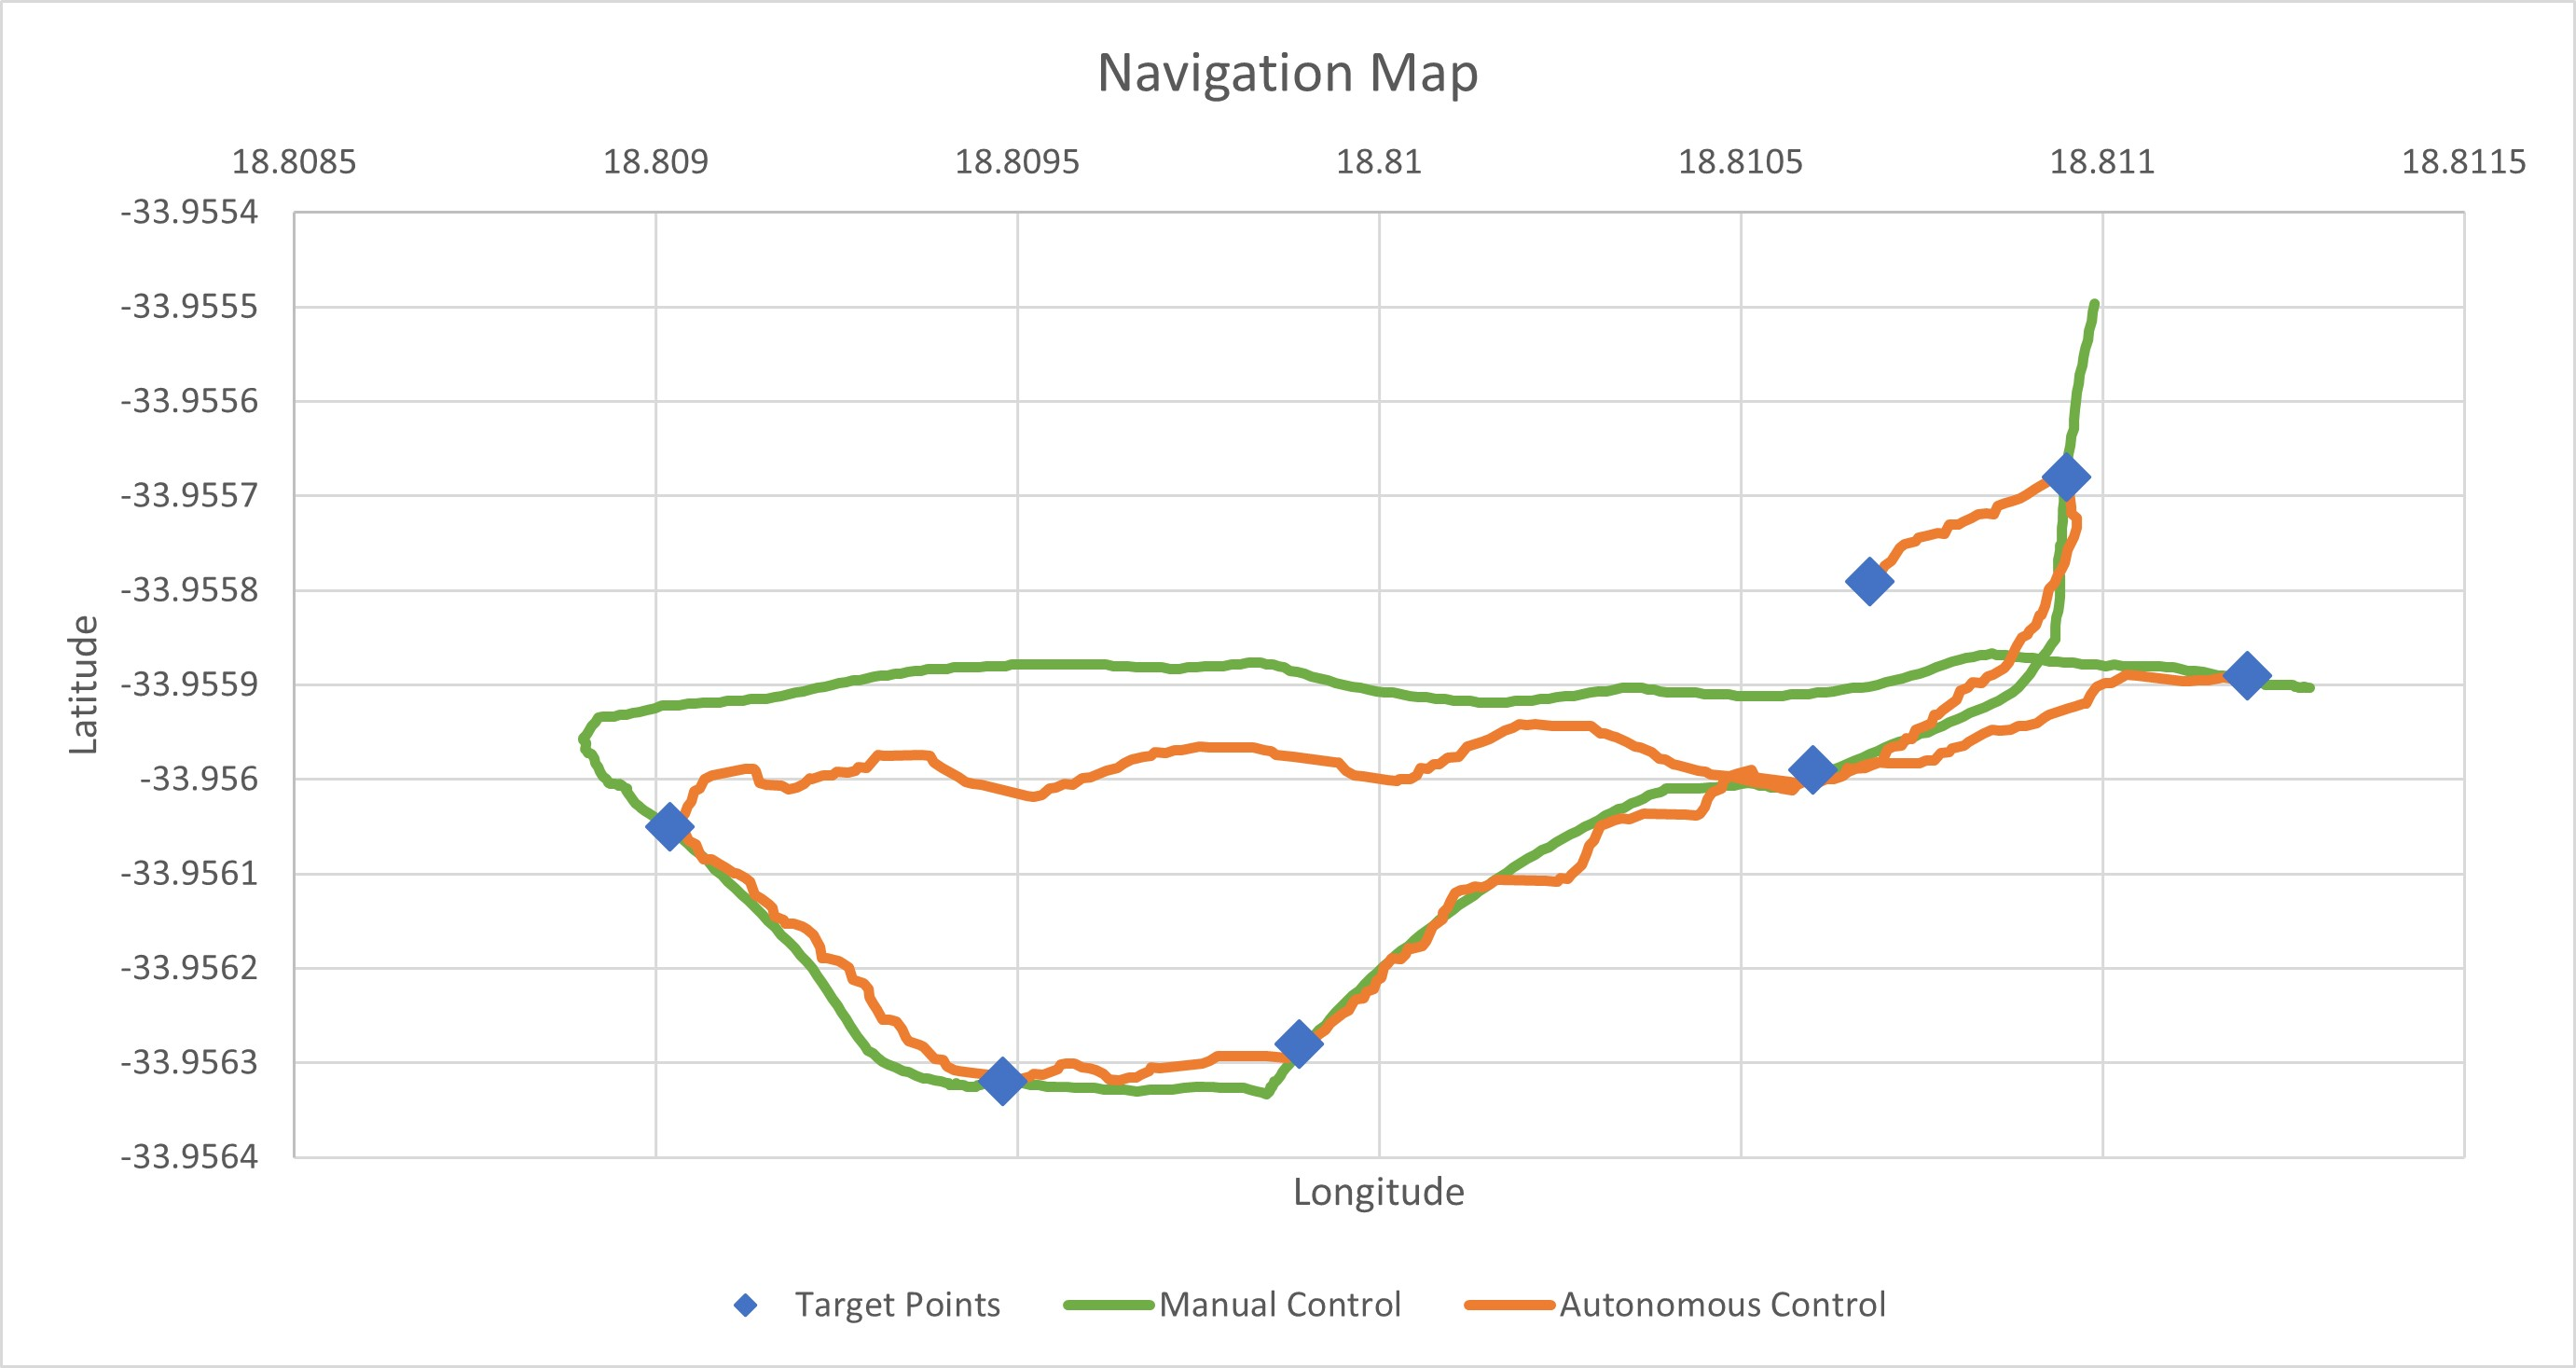
\includegraphics[width = 0.84\linewidth]{figures/graphMap.jpg}
		\caption{Map of Test 1.}
		\label{graph:4:Map}
	\end{center}
\end{figure}
\vspace{0.8cm}
\subsection{Results}
After all the testing had been completed, the results could be analysed and assessed to determine the validity and performance of the control system. The results will be discussed with the aid of graphs draw from the data collected during the tests. The performance of the control system will be determined by how accurately it stays on the course to the target location and the validity of the system will be determined by if the vessel reached the target points. \par
The initial autonomous test carried out was successful in that it navigated to the points after some time. However, there was a lot lacking as the navigation was very far off course for large portions of the test. Figure \ref{graph:4:Map} shows the route of the manual test and the first autonomous test, the manual test is also shown in Figure \ref{graph:4:Map2} as a reference point between the two autonomous tests. It can be seen in Figure \ref{graph:4:Map} that the vessel does navigate to the points but there are large unnecessary loops that the vessel travels. This points to the navigation system being valid but very inaccurate. Once the data could be analysed, it became apparent that the inaccuracy was caused by the compass having lost calibration. The data showed that even on the long looping path, the compass reading was within \SI{40}{\degree} of the target bearing which was clearly incorrect. It appears that the compass had accurate calibration in the approximate range of \SI{350}{\degree} to \SI{150}{\degree}. This is further backed up by how the vessel always followed a long loop until the point was within this range, at which point it would successfully navigate to the point. Due to the inaccuracy of the test and the underlying cause being a faulty sensor and not a flaw in the system, another test was planned.\par
\vspace{0.6cm}
The second autonomous test was conducted under less than ideal conditions with a steady wind blowing from the South East. However, even under these conditions the system performed well and navigated to within the acceptable distance of \SI{7}{\metre} of each point. Figure \ref{grph:4:distance} shows the distance to the targeted point as the time elapsed. It can clearly be seen that the vessel was a path of steadily decreasing the distance to the point until arrival. The only exception is just before arriving at point 5, the distance slightly increases. This was due to the vessel heading straight at a buoy. The vessel was pushed off against the buoy to avoid contact the system handled the disruption by correcting its course and navigating back to the target.\par 
The disruption can further be seen in Figure \ref{grph:4:BearingError} with a large spike in the difference between the vessel bearing and the target bearing. This spike is corrected and the course is resumed. The other large spikes on Figure \ref{grph:4:BearingError} all correlate with the arrival at a point upon which the target is moved to the next point and a large error occurs before the system can turn itself and navigate to the next point. Another trend of Figure \ref{grph:4:BearingError} shows that the vessel settles around \SI{10}{\degree} off from the target bearing. This is not a large static error and could be tuned out in the control system, however more tests would need to be conducted to ensure that the static error is not caused by external factors such as the steady wind during the test. \par
The steady error can also be seen in Figure \ref{grph:4:2bearings} where the vessels bearing is mostly just above the target bearing. However, Figure \ref{grph:4:2bearings} also clearly shows that the vessel reacts well to changes in the target bearing and tracks the target bearing closely with minimal overshoot. The sudden change of bearing between points 4 and 5 in Figure \ref{grph:4:2bearings} is due to the vessel turning across the \SI{360}{\degree}\\\SI{0}{\degree} turnover point. \par
Another trend that can be seen across both Figures \ref{grph:4:BearingError} and \ref{grph:4:2bearings} is that the vessel has a large amount of oscillation and is often referred to as 'fish tailing'. The oscillations can be explained by the thrusters that were used. Even with the increase in voltage the thrusters were underpowered in comparison to the weight and shape of the vessel. This meant that the steering was slow to respond and the progressive steering implemented was not very noticeable. To further compound on the issue, it became apparent during the manual test that one thruster produced slightly more thrust than the other leading to a slight drift when both thruster were fully powered and also allowed the vessel to be more manoeuvrable when turning one direction as opposed to the other. However, given these oscillations when looking at the overall navigation map of Figure \ref{graph:4:Map2} the path of the vessel is relatively straight in the overall distance travelled. Figure \ref{graph:4:Map2} shows the effect the wind had with a small effect evident on the route between points 2,3 and 4 with the vessel into the wind. However, between points 5 and 6, when the vessel was travelling mostly with the wind, it had a large impact and blew the vessel off course and the system had to correct to finally reach point 6.\par
Overall the system performed well with less than ideal weather conditions and underpowered and slightly uneven thrusters. Given these, the system still managed to navigate to within the prescribed allowable distance and maintain a relatively straight route between all points and not doing any unnecessary navigation. The system could easily be upgraded to a larger more appropriate vessel with the required thrust with little alterations.

\begin{figure}
	\begin{center}
		\begin{subfigure}{0.8\linewidth}
			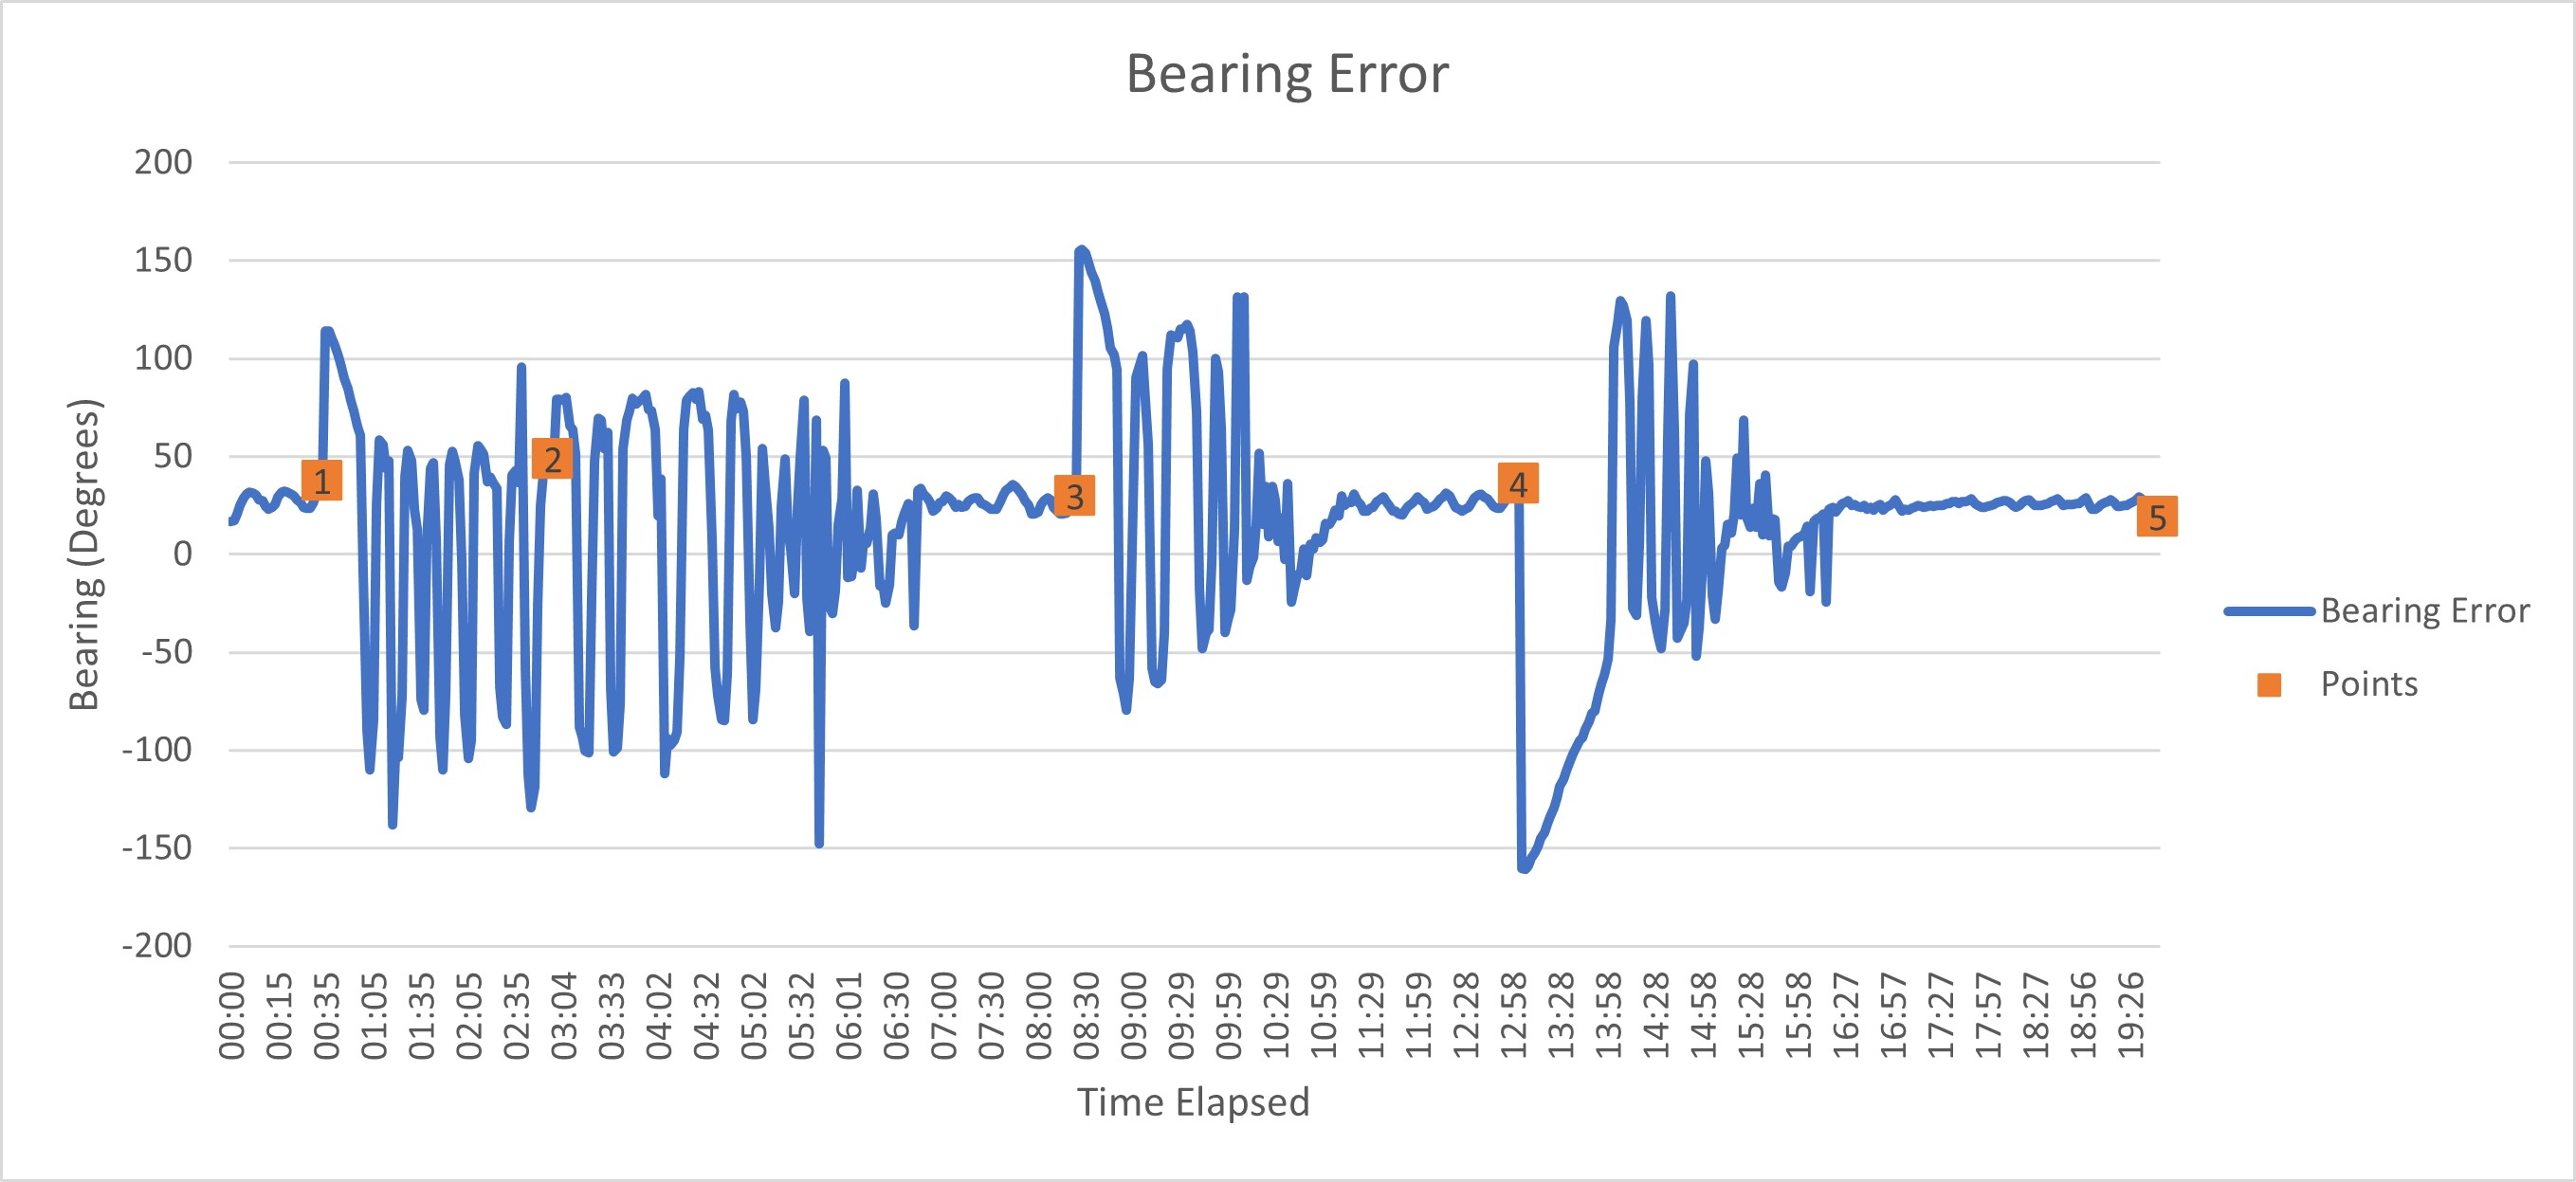
\includegraphics[width = \linewidth]{figures/graphBearingError.jpg}
			\caption{Bearing Error.}
			\label{grph:4:BearingError}	
		\end{subfigure}
		\begin{subfigure}{0.8\linewidth}
			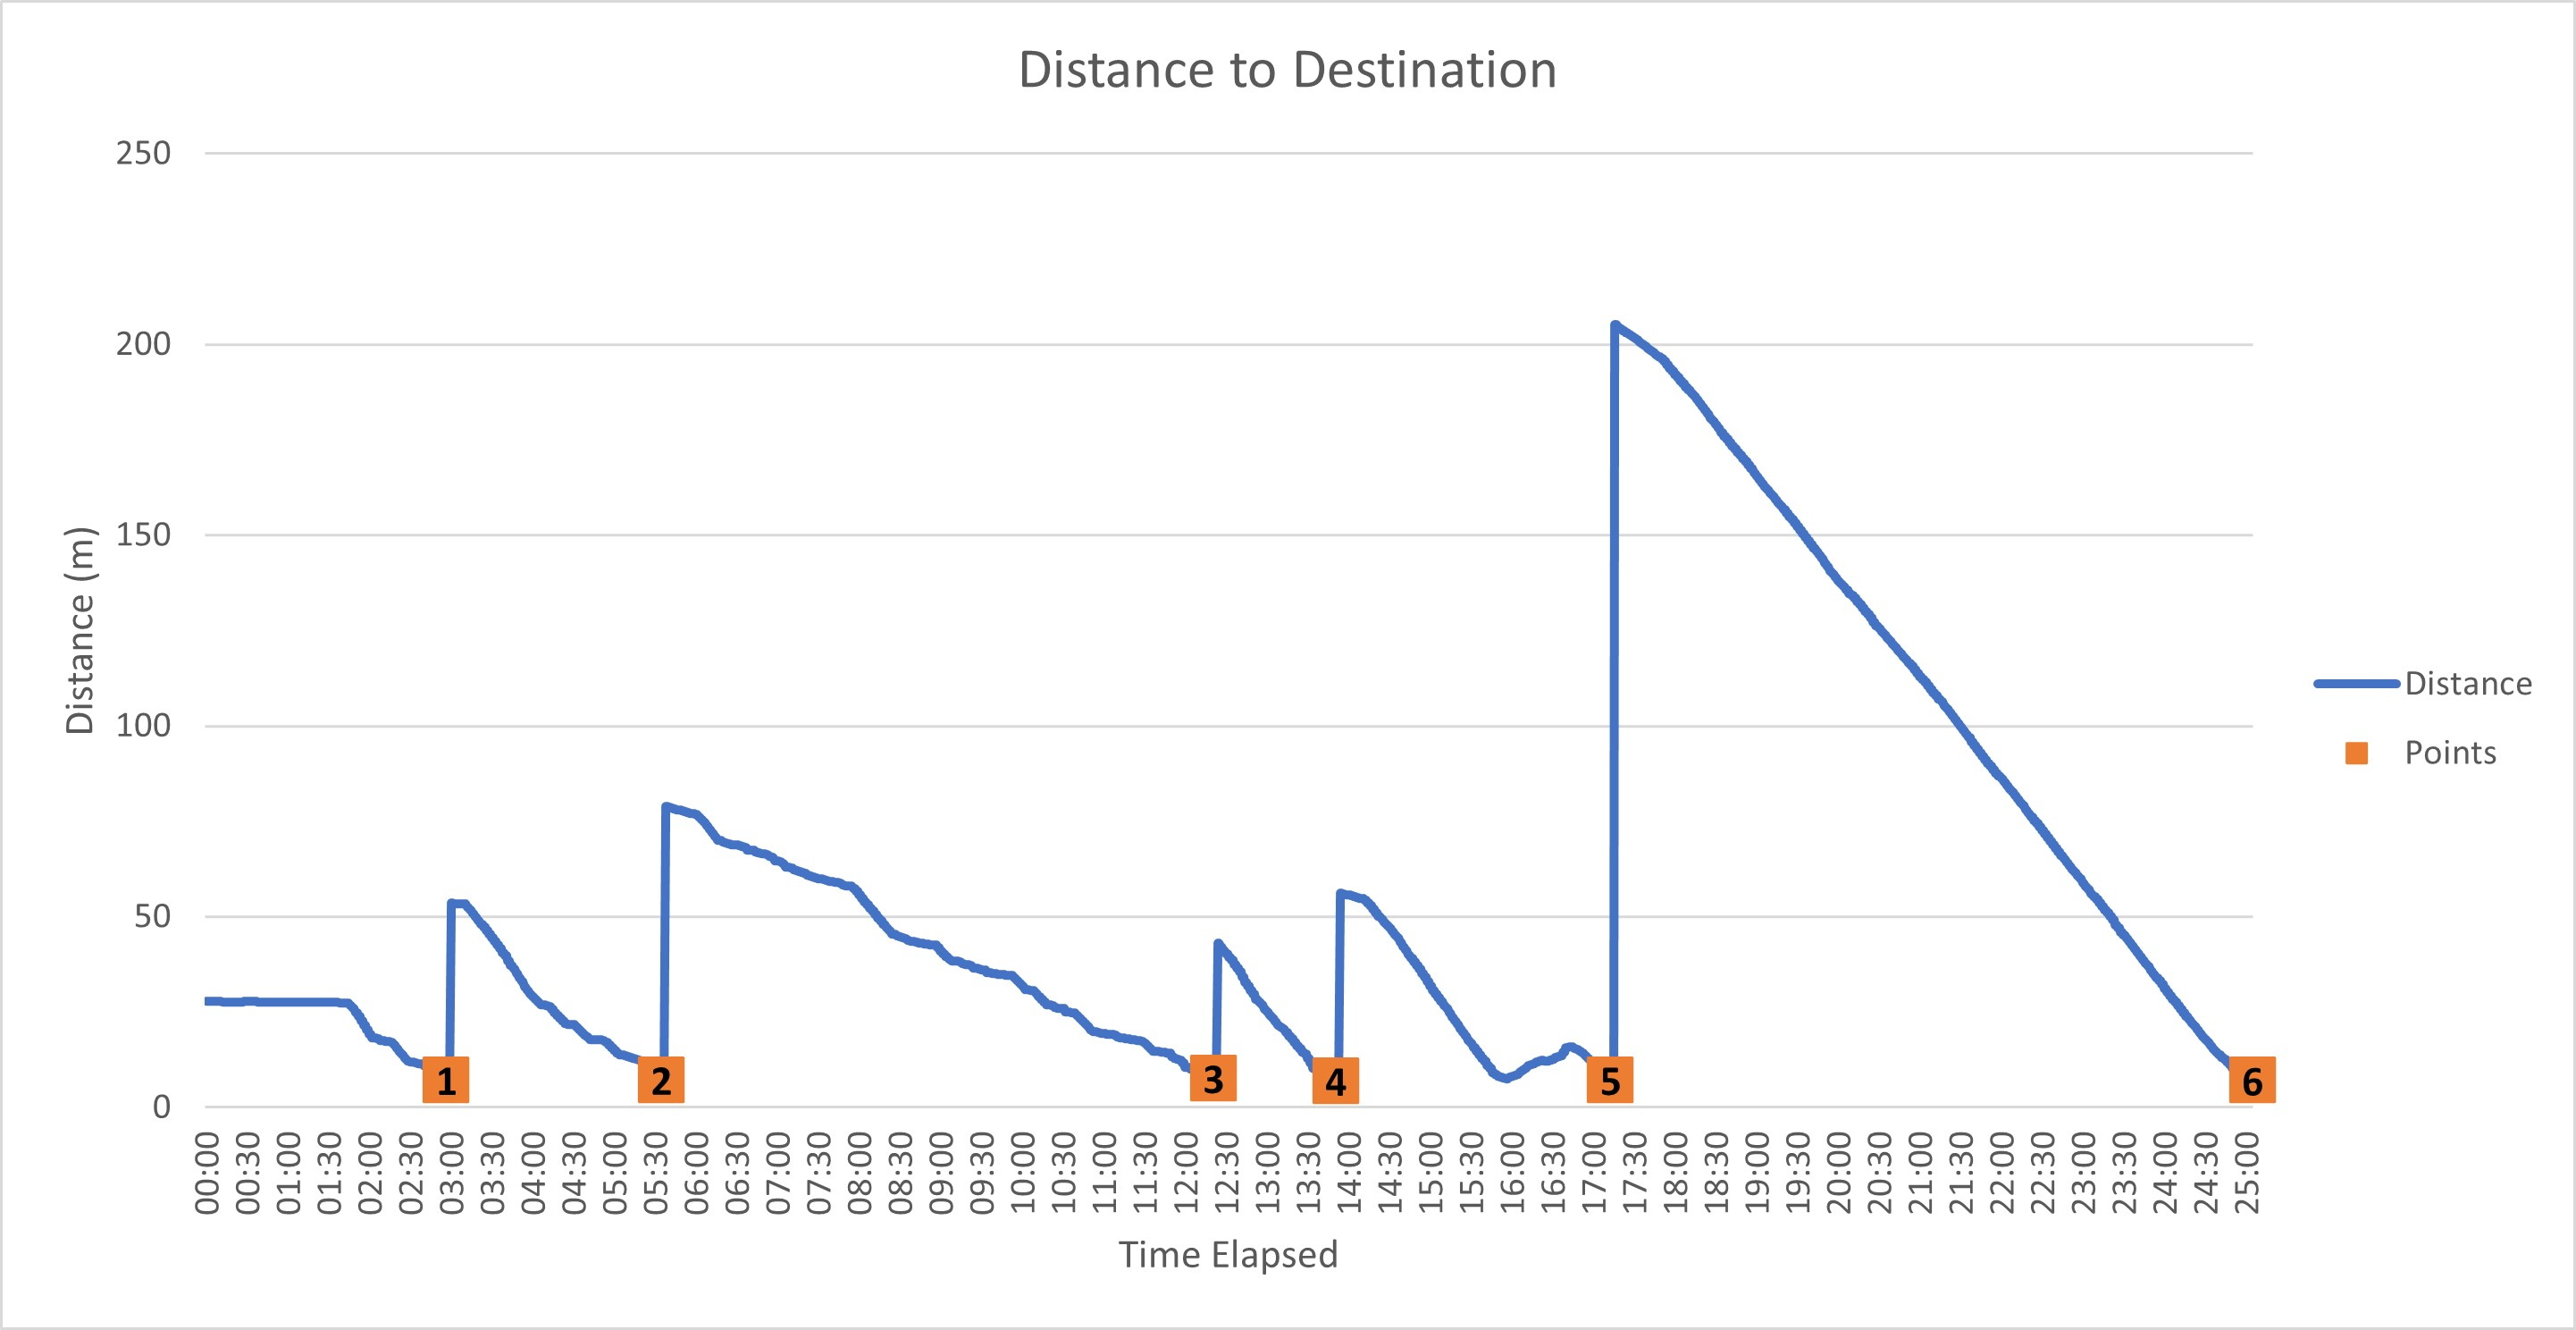
\includegraphics[width = \linewidth]{figures/graphDistance.jpg}
			\caption{Distance to Target.}
			\label{grph:4:distance}	
		\end{subfigure}
		\begin{subfigure}{0.8\linewidth}
			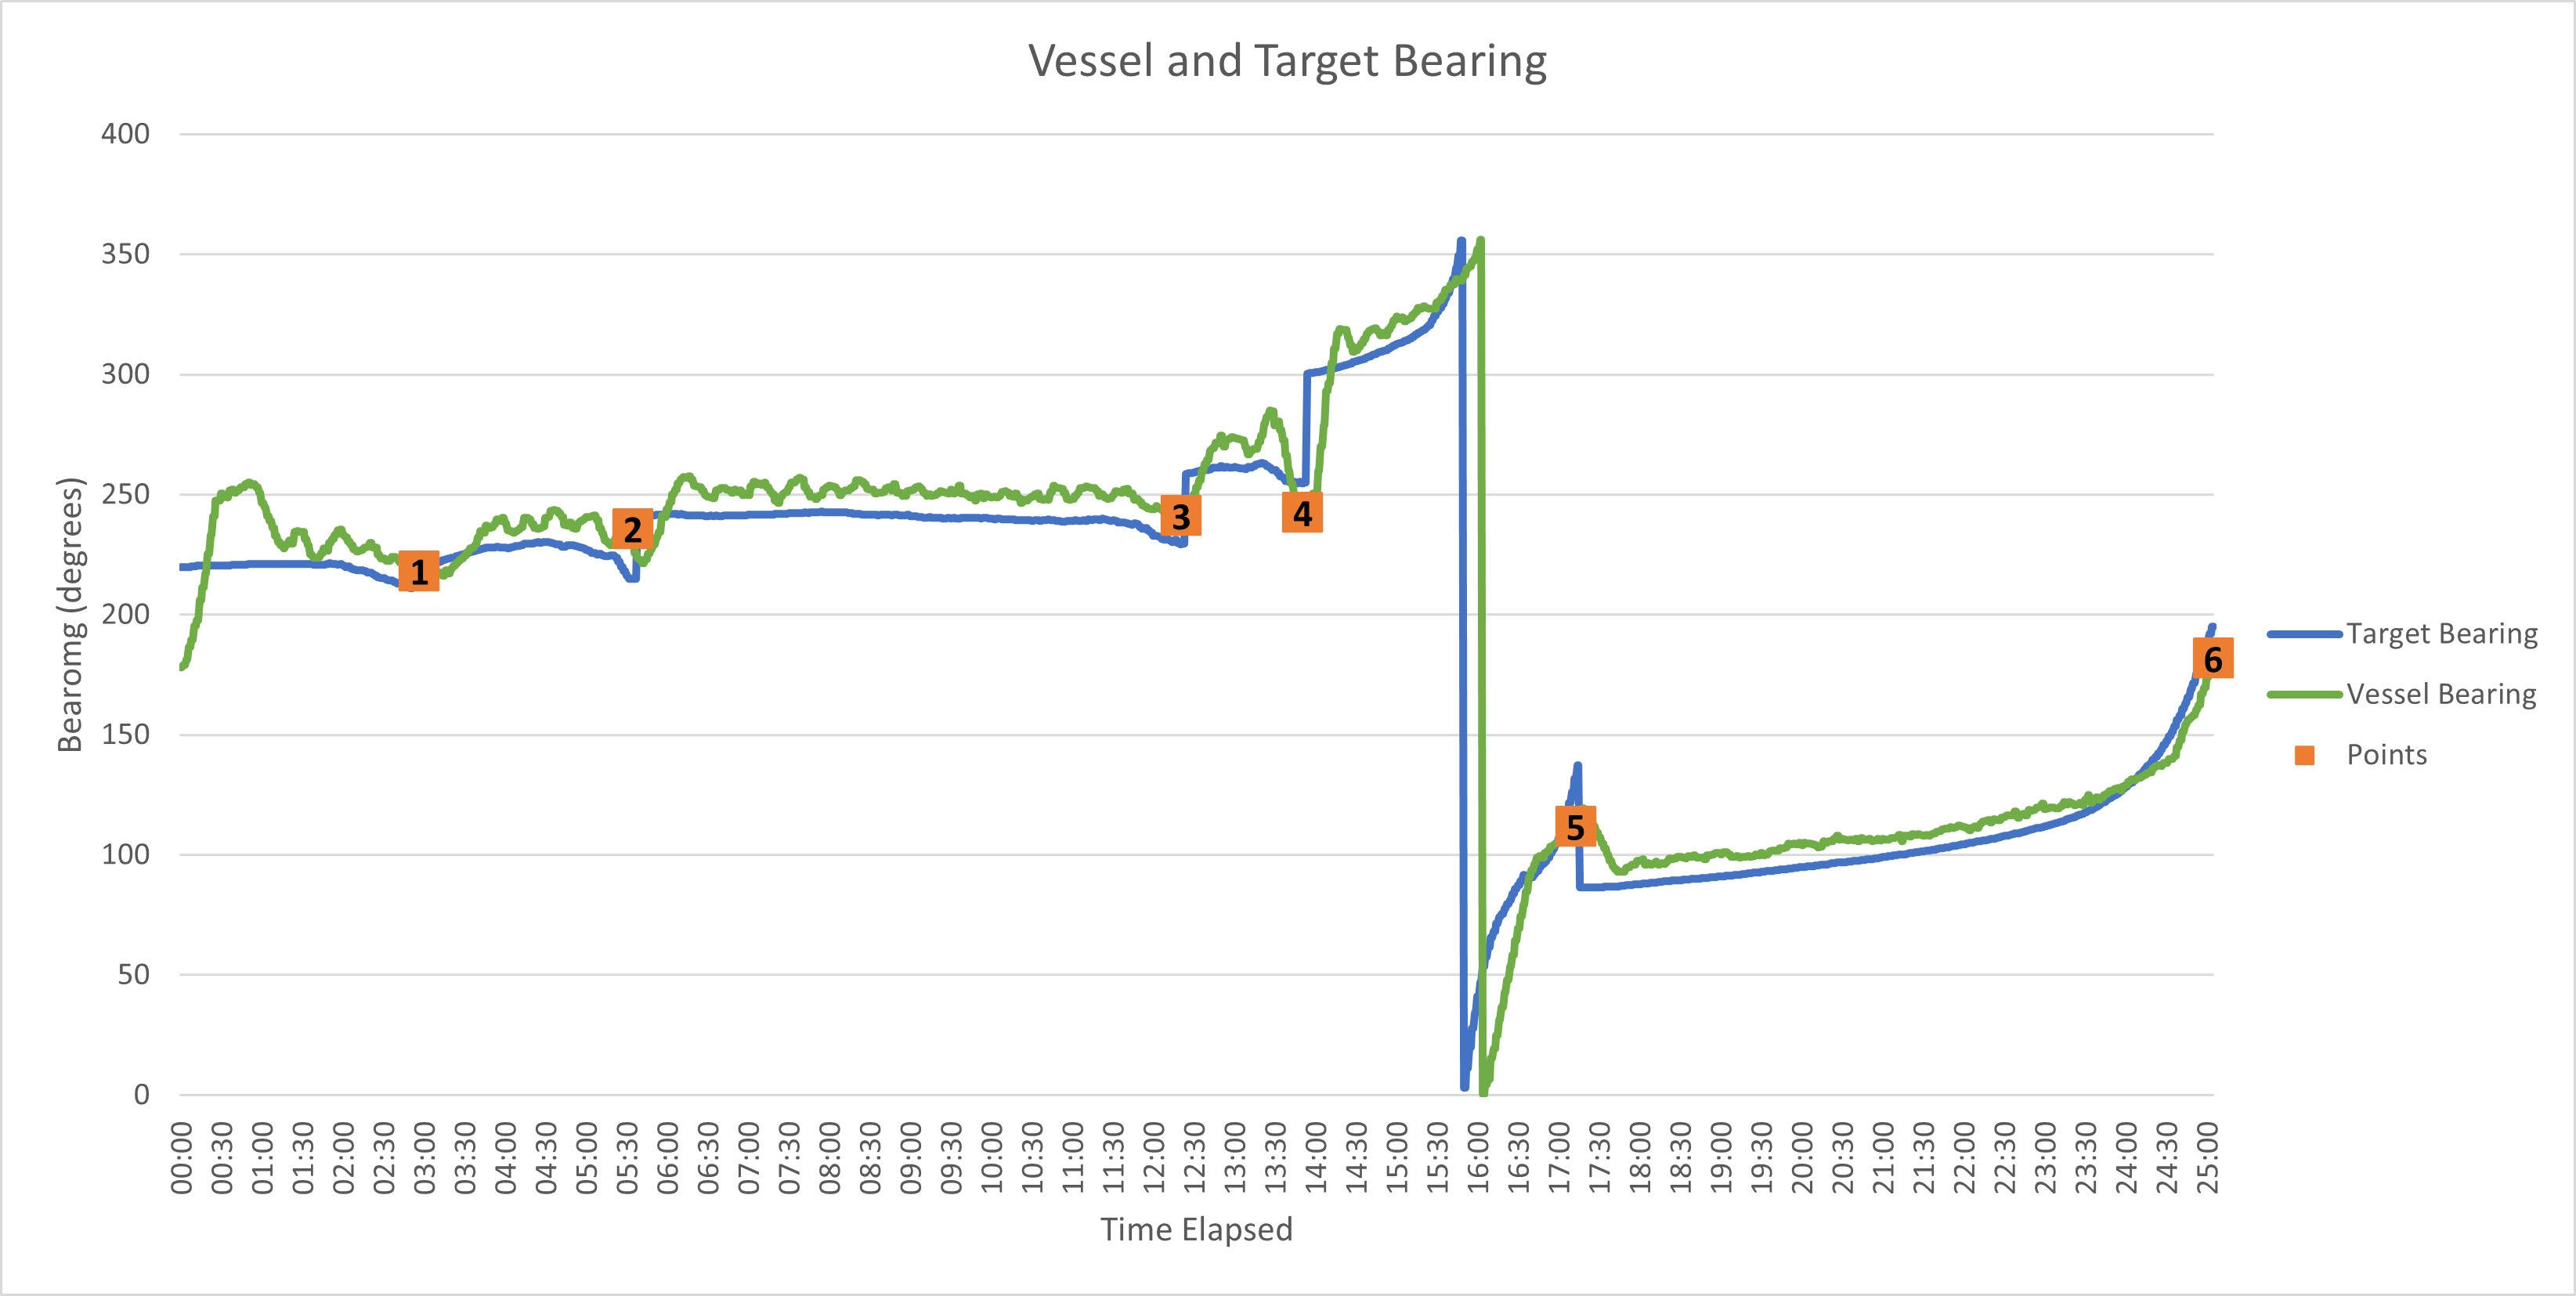
\includegraphics[width = \linewidth]{figures/graphBearings.jpg}
			\caption{Bearings Comparison.}
			\label{grph:4:2bearings}	
		\end{subfigure}
		\caption{Results of the PWM output displayed on an oscilloscope.}
		\label{fig:4:Results}
	\end{center}
\end{figure} 
\begin{figure}[hb]
	\begin{center}
		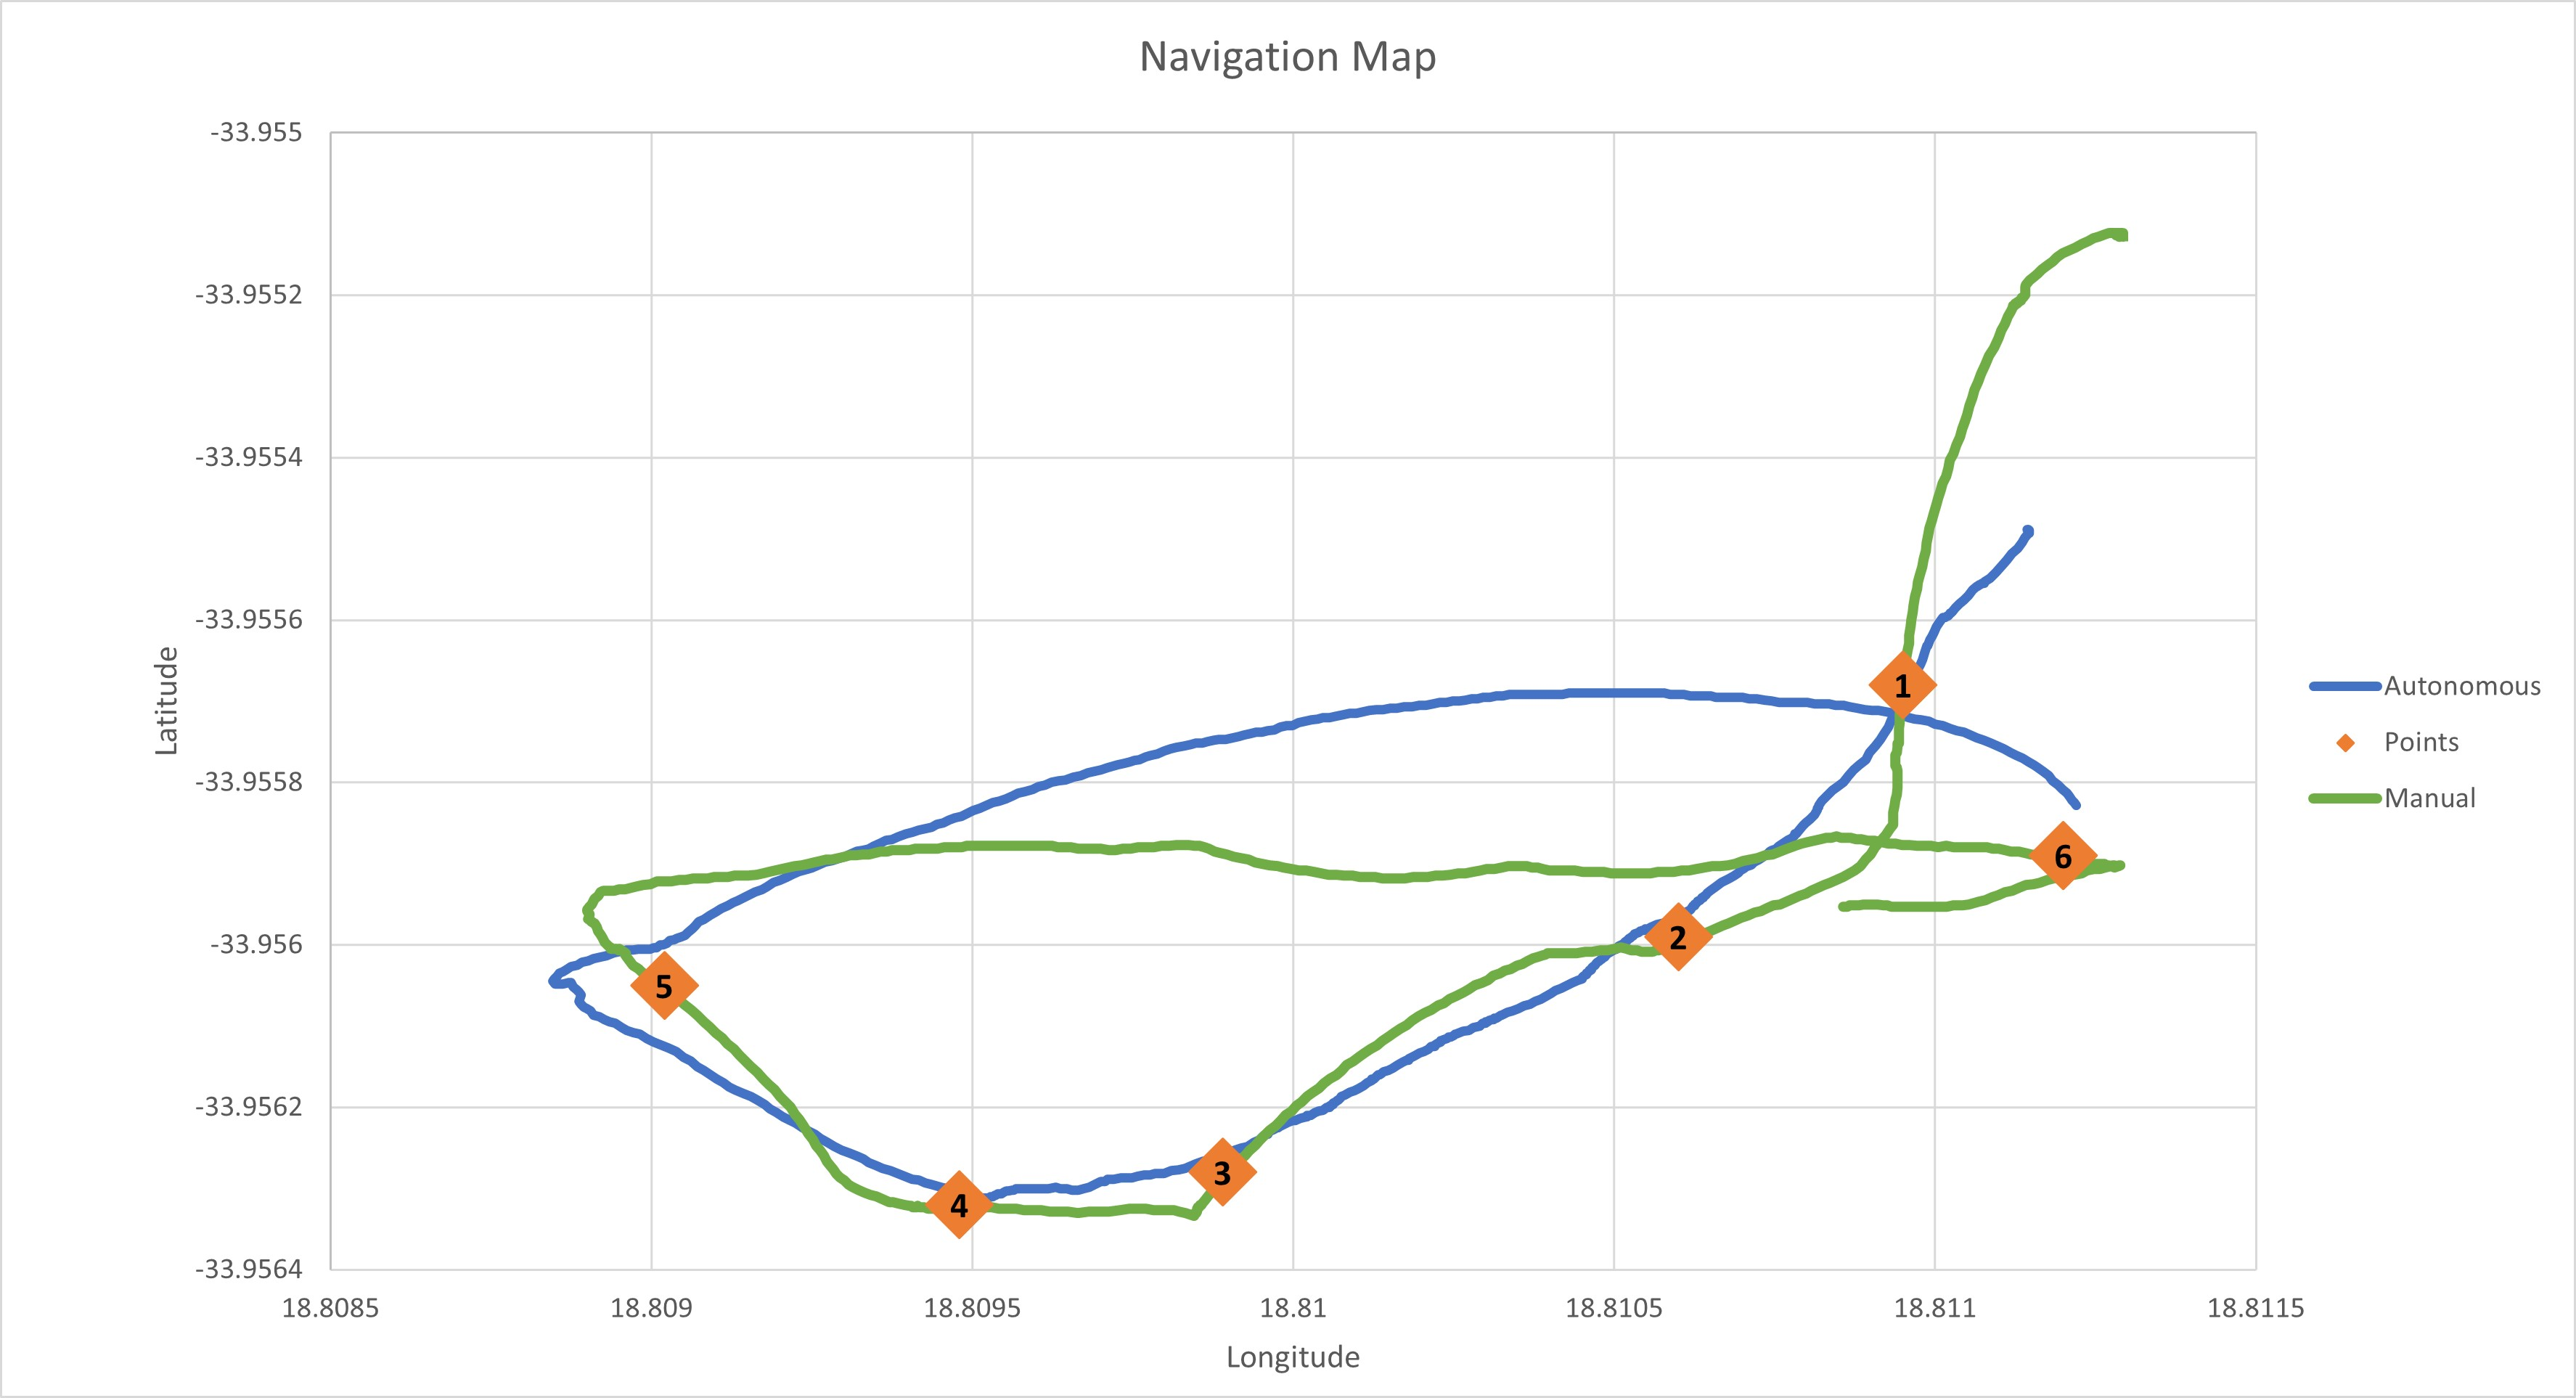
\includegraphics[height=0.8\linewidth, angle = 270]{figures/graphMap2.jpg}
		\caption{Map of Test 2.}
		\label{graph:4:Map2}
	\end{center}
\end{figure} 